\chapter{Clustering and Kinetics}
\label{chap:clustering_kinetics}

Macrostates, collections of microstates that share similar characteristics, are a useful tool in the study of any system, for instance, in setting up coarse-graining models. For proteins in particular, with a small enough set of macrostates one can usually deduce the folding pathway with even a rudimentary kinetic model. This poses a problem for a system with many degrees of freedom; how does one go about finding the relevant macrostates in the first place? In this chapter we develop a plan for partitioning the microstates into broad, meaningful macrostates from time-series data or detailed microstate information. We begin with an outline of the methodology and elaborate on the details through two models: a kinetic trajectory taken from a frustrated Langevin system and a small, idealized $\beta$-hairpin embedded on a two-dimensional lattice. We will see that the macrostate clustering method developed here provides a robust tool in the analysis of dynamical systems. 

\section{Macrostate Clustering}
\label{sec:clustering_outline}

In theory, the equations of motion along with initial conditions impart complete knowledge of any system. In reality, the situation is more complex. Few systems can be solved analytically, and these solutions are often idealized models of the underlying mechanics. Topological characterizations can usually be made (such as Lyapunov exponents), but these convey a solution only in the broadest sense. What is needed is geometrical measure, a way of partitioning the phase space to a more manageable subset. If our system is near or at thermal equilibrium this is tantamount to  clustering the microstates into physically meaningful macrostates. The idea is not new, many of the early pioneers of biophysical models have been advocating different methodologies for macrostate classification.\cite{ozkan_computing_2003, zhou_minimum-reaction-flux_2008} It would be useful to have a general purpose algorithm for constructing the macrostates from information obtainable from the equations of motion, or a statistical description of the system.

In this chapter we propose a viable method for macrostate clustering (MSC for short). The MSC algorithm takes as input a kinetic trajectory and a single parameter. We convert the kinetic trajectory into a Markov matrix and use its eigenvectors to make this classification. Since an embeddable Markov matrix is a mapping from a system of linear first-order differential equations, the MSC algorithm can be considered a first-order approximation to the motion.

With a system specified by its Hamiltonian $\HAM$ and intensive properties, the first step is a suitable identification of the microstates $\{\xi_1, \xi_2,\ldots, \xi_N \}$. For continuous systems, the accessible state space must be partitioned.\footnote{In practice this is easily adjustable even after a trajectory has been obtained and does not change the results of the MSC algorithm greatly. With a finer partitioning method, more resolution is obtained at the cost of under-sampling. This consequently increases the running time.}  A trajectory is obtained by integrating the equations of motion, making note of the conformation at equal time intervals. An incidence matrix is formed by counting the number of times microstate $\xi_i$ moved to $\xi_j$. This matrix can be converted to a proper Markov matrix by normalizing the row sums. Alternatively, if one had complete knowledge of the microstates and the transition rates between them, one could convert this matrix into a Markov matrix without the loss of any information, that is, the Markov matrix is a snapshot of a continuous time Markov process. With Markov matrix $\B{M}$, compute the Schur eigendecomposition
\begin{equation}
  \B{M} = \B{V \Gamma V}^{-1}
\end{equation}
where $\B{\Gamma}$ is a diagonal matrix with  eigenvalues $\lambda_1 \geq \lambda_2 \geq \ldots \geq \lambda_N \geq 0$. Since $\B{M}$ is a Markov matrix, $\lambda_1=1$ corresponds to the slowest mode of relaxation of the system, \ie the steady-state. The other eigenvalues, being smaller, represent faster modes of relaxation (see Section \ref{sec:markov_matrix} for more details on Markov matrices). The influence of the modes on the relaxation of the system is exponential $\propto e^\lambda$, thus the slower modes not only represent the dominant flows of the system, they are less influenced by the initial conditions. This makes them prime candidates for macrostate discovery. The fastest mode included in this consideration is the single free parameter in the MSC algorithm, $\phi$. Let this parameter $0 \le \phi \le 1$ be the eigenvalue threshold cutoff. Take a cut of the eigenvector matrix $\B{V}$, retaining only those vectors where $\lambda_i > \phi$. At $\phi=1$ only steady-state is retained, while at $\phi=0$ all modes have equal influence.  If the number of eigenvalues remaining is $k$ then 
\begin{equation}
  \B{U} = \text{cut}(\B{V})
\end{equation}
is a $N$ by $k$ matrix. While the columns are the eigenvectors, each row $u_i \in \B{U}$ represents microstate $\xi_i$ contribution to the remaining modes. We call the vectors $u$ the eigenflows of the system. We can imagine each of the $N$ vectors as points in the space of $\mathds{R}^k$. This gives the central idea behind the MSC algorithm. Microstates should be grouped into macrostates by clustering their eigenflows. Eigenvectors are unique up to a sign, so the clustering must take this into account. Formally, we are looking to define a metric $\B{g}(u_i, u_j)$, such that two eigenflows belong to the same cluster if, for some small $\epsilon$ 
\begin{equation}
  \B{g}(u_i, u_j) = \norm{ u_i - u_j } < \epsilon
  \label{eq:egienflow_metric_general}
\end{equation}

The idea has physical appeal, points near a local minima in phase space should all have similar eigenflows. Transition points in the system should be different, they should split the flow across the boundaries giving distinct components in their eigenflows compared to the local minima. In practice we found the main stumbling block was twofold: the choice of a proper metric (Equation \ref{eq:egienflow_metric_general}) and a suitable algorithm to group the elements into clusters implied by $\B{g}_{ij}$. Initially we choose the Euclidean metric $\norm{\cdot}_2$ and used various clustering algorithms to group the states. The method was only partially successful. The greatest shortcoming was the introduction of several new ad-hoc parameters into the system from the clustering algorithms. We eventually settled on a simpler classification that relied on no new parametrization. Let
\begin{equation}
  \sgn(u) = \brackets{ \sgn(u_1),  \sgn(u_2), \ldots, \sgn(u_k) }
\end{equation}
be the sign signature of a vector, where we define 
\begin{equation}
\sgn(x) = \piecewisebrace{
 \begin{array}{r l l}
   -1 & : & x < 0 \\
    1 & : & x \ge 0 %\text{otherwise}
 \end{array}
 }
\end{equation}
%
Two microstates belong to the same cluster (and hence macrostate) if and only if their sign signatures are equal. We assign each of the microstates $u_i$ to clusters in $\mathcal{C}^\prime = \braces{ c_1, c_2, \ldots, c_{2^k}}$. Not every cluster will be populated, since it is possible for $2^k > N$. Let $\mathcal{C}$ be the set of non-empty clusters and $\abs{\mathcal{C}}$, $\abs{c_i}$ count the number of clusters and the number of microstates within cluster $c_i$ respectively.

\subsection{Quasi-steady-state}

Once the clusters have been identified, we can present a macroscopic version of the original Markov matrix. Since macrostate behavior is often dominated by rare transitions between macrostates, we will assume that each macrostate relaxes to a local steady-state. We call this the quasi-steady-state. For each cluster we first compute the quasi-steady-state transition probability. 

Let $\B{M}_{c_i}$ be the square matrix with $\abs{c_i}^2$ elements that are pulled from cluster $c_i$.
This cluster is approximated as an isolated system, as we've only retained the flows within this cluster. We row normalize the matrix, discarding any rows (and their associated column) where the row sum is zero. Such states are possible within a transient cluster since it is conceivable that the trajectory from a fixed microstate does not flow to any other microstate in the cluster. The quasi-steady-state vector $\pi(c_i)$ is given by the left-eigenvector with eigenvalue one of the reduced renormalized Markov matrix
\begin{equation}
  \pi(c_i) \B{M}_{c_i} = \pi(c_i)
\end{equation}

Once we have computed the quasi-steady-states we use them as initial conditions to approximate macrostate behavior. Over a single time step these initial conditions will flow into other clusters giving us macrostate kinetics. Let $b_i$ be a vector of initial conditions from the full system. This vector has $N$ elements that correspond to those in $\pi(c_i)$, \ie it is the initial condition of quasi-steady-state for cluster $c_i$ and zero for all the elements of the other clusters. We start the system in $b_i$ and advance it one time step $b_i \B{M}$ to get the Markov macrostate matrix $\B{S}$.
%
\begin{equation}
  \B{S}_{a b} = 
  \sum_{i \in c_b}^{\abs{c_b}} 
  \paren{ b_a \B{M} }_{i} 
  \label{eq:macrostate_cluster_matrix}
\end{equation}

The matrix $\B{S}$ gives us new macrostate information. In addition to simply identifying the macrostates, the matrix identifies kinetic pathways by giving us the transition rate to each cluster. By starting at some set of initial conditions, we can trace a pathway along the clusters by continuously applying $\B{M}$ to the set. From here we can discard irrelevant clusters to a particular problem, and identify intermediate macrostates along the way. The identification of intermediates would be difficult with the original matrix; no single intermediate microstate dominates the statistics. When the states are clustered together, their similar eigenflows tend to move in tandem. These newly identified macrostates could present a new reaction coordinate or kinetic pathway. In the two subsections below, we apply the formalism to two illustrative cases.

\section{Frustrated Langevin Walk}

In this example we work directly with time-series data from a kinetic trajectory. The trajectory is obtained by integrating the equations of motion of a random walk in an external field. We will see that only the time-series data are needed, knowledge of the Hamiltonian or a suitable reaction coordinate is not required to determine the macrostate classification.  This example is particularly useful in view of the popularity of molecular dynamics (MD) simulations in the biophysical community.\cite{karplus_molecular_2002} In MD simulations, one often has many degrees of freedom, hence developing a general model is often a non-trivial task. The ability to partition the conformational space into physically relevant macrostates of lower dimension would greatly facilitate a deeper understanding of the system.

We model a particle in a viscous fluid subject to stochastic noise in a Langevin-like equation.\cite{coffey_langevin_2004} There are kinetic traps - minima in the potential that localize the motion until the particle can escape by thermal diffusion. Because of this, we call the system a frustrated Langevin walk (FLW). 

The traps are modeled as Gaussian wells. To simplify the expression of the equations of motion we define an isotropic Gaussian well that is centered at $(x_R, y_R)$ by 
\begin{align}
  L(x_R,y_R) &= -\exp \paren{ - \sqrt{ (x-x_R)^2 + (y-y_R)^2 } } \\
  \intertext{The potential, shown in Figure \ref{fig:clustering_smooth_map_traj}, is the contribution of three wells}
  V(\B{x}) &= L(0,0) + L(2,2) + L(0,-2)
  \label{eq:FLW_potential}
\end{align}
with $\B{x} =(x,y)$. Since the potential at a given point is the sum of the Gaussian wells, the depth at each of the three minima have the relation $V(0,0) < V(0,-2) < V(2,2)$. 

In addition to the potential, the particle is subject to stochastic noise and viscous damping
%
\begin{equation}
  m \B{\ddot x} = - \nabla V(\B{x}) - \lambda \B{\dot x} + \B{\eta}(t)
  \label{eq:FLW_force_eq}
\end{equation}
The dot notation indicates a derivative with respect to time. The damping coefficient  $\lambda$, is a measure of the frictional forces acting on the system proportional to the velocity. The stochastic term $\B{\eta}$, is an approximation to the microscopic collisions the particle would experience in a real fluid. The force has a correlation time of
\begin{equation}
  \avg{ \eta_i(t) \eta_j(t') }
  =
  \frac{ 2 \lambda }{\beta} \delta_{i,j} \delta(t- t')
\end{equation}
%
We choose the parameters $\beta=m=1$, $\lambda=0.07$ as they were sufficiently weak to bound the motion, but strong enough to occasionally facilitate a transition over the potential barriers. We integrated the system for a total time of $t_{\text{max}} = 10^6$ using a time step of $\Delta=0.2$ with a standard Runge-Kutta 4th order integrator.\footnote{
  Integrating a stochastic differential equation properly is a subtle, difficult task. Since most integration schemes rely on a Taylor expansion, it becomes problematic when there are force terms that are nowhere differentiable. In general, one must expand with the time-ordered exponential $T$
  \begin{equation}
    T \brackets{\exp{
        i \int_0^{\delta t} \mathcal{L}(s) d s 
    }}
  \end{equation}
  where $\mathcal{L}$ is the Liouvillian.\cite{suzuki_general_1992} Since our focus is on the method of macrostate approximation, we estimate the stochastic force by adding a random perturbation to the force each step of the integration. A deeper study of the system in question would require a proper handling of this issue by considering a suitable time-ordered integration scheme.\cite{goldman_nth-order_1996, ricci_algorithms_2003,ciccotti_deterministic_2004}
} 
%
The trajectory $\mathcal{T}$, is an ordered list
\begin{equation}
  \mathcal{T} = \{ \B{x}_{t_0}, \B{x}_{t_1}, \ldots, \B{x}_{t_\text{max}} \}
\end{equation}
%
A sample trajectory is plotted in Figure \ref{fig:clustering_smooth_map_traj}. The accessible coordinate space $\{\xi_1, \xi_2,\ldots, \xi_N \}$, is given by discretizing the interval $\B{x} \in [-4,4]$ into $N=45^2$ squares . For a given position, let $\Xi(\B{x})$ return the discretized position in coordinate space. For example, if $\B{x}_i \in \xi_j$ then $\Xi(\B{x_i}) = \xi_j$. We choose a lag time of $5 \Delta$ to simulate the collection of time-series data collected at larger intervals than the integrating time-step. Next we computed an incidence matrix $\B{C}_{ij}$. This matrix counts the number of times over the lag time the trajectory went from $\xi_i$ to $\xi_j$ 
\begin{equation}
  \B{C}_{ij} = 
  \sum_{i=5}^{ {t_{\text{max}}}/{\Delta}} \delta(\Xi(\B{x}_{t_{k-5}}),  \xi_i) \ \delta(\Xi(\B{x}_{t_{k}}),  \xi_j)
\end{equation}
%
A Markov matrix $\B{M}$ is constructed from the incidence matrix by normalizing the row sums
\begin{equation}
  \B{M}_{ij} = \frac{ \B{C}_{ij} } {\sum_k \B{C}_{kj}}
\end{equation}
%
It is worth nothing that the resulting Markovian matrix is only a linear approximation to the actual dynamics. Especially in the regions between pairs of the wells the may not hold. However, it is a useful first-guess a the transition rates that can later be refined. The Markov matrix was diagonalized and clusters were created with an eigenvalue cutoff of $\phi = 0.85$. This partitioned the conformational space into four clusters, shown in Figure \ref{fig:clustering_smooth_map_cluster_loc}.

\begin{figure}[tb]
  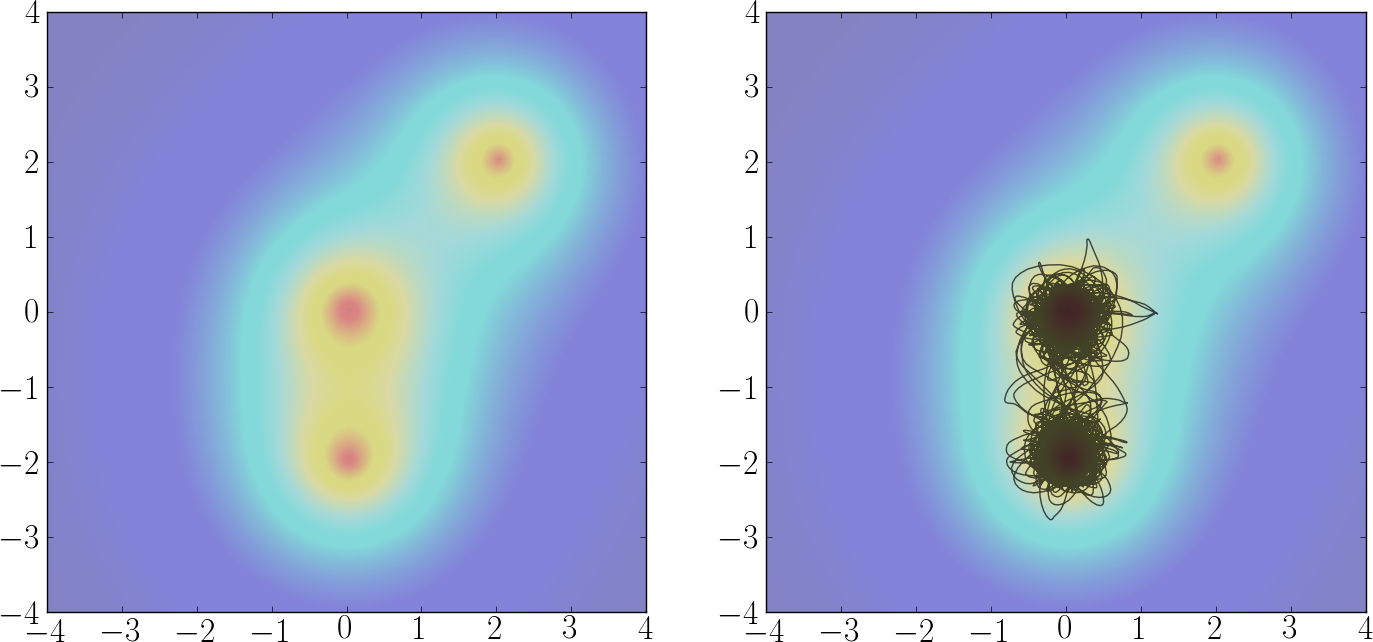
\includegraphics[width=.8\textwidth]{supplement/smooth_potential_cluster/pictures/smooth_potential_traj.png}
  \caption{(Left) Contour map of the three well Gaussian potential, Equation \ref{eq:FLW_potential}. (Right) A sample ($0.2 t_{\text{max}}$) of the FLW trajectory shown by integrating Equation \ref{eq:FLW_force_eq}. The motion is localized in the wells, escaping only when random fluctuations push it over a potential barrier.}
  \label{fig:clustering_smooth_map_traj}
\end{figure}
%
With the clusters identified, we permuted the Markov matrix to reflect our knowledge of the clusters. In Figure 
\ref{fig:clustering_smooth_map_markov_permutes} we see that the original matrix has no particular structure, while the permuted matrix shows a nearly block diagonal structure. The non-zero elements off the block diagonal indicate transitions between the clusters, while those within the block indicate movement within the cluster. The macrostate approximation identified all three local minima and the largest crossing barrier. Our choice of $\phi$ was not arbitrary, it was selected to be large enough to grab the semi-stable states, yet small enough to have broad macrostates. When $\phi$ is lowered, the state space partitioned into finer clusters. This may or may not be helpful in determining a kinetic pathway, the macrostates need to be connected to a physically relevant set of macro coordinates. Therefore, while a lower $\phi$ gives more information, not all of it is useful. For example, when a slightly lower $\phi$ is used there are two new macrostates: the first is a barrier crossing between the bottom wells (labeled $c_1$ and $c_2$ in Figure \ref{fig:clustering_smooth_map_cluster_loc}), and the second is a ring shaped boundary around the upper well $c_0$. The first is well-understood, it clearly represents the boundary between two more dominant macrostates; this barrier is useful for characterizing the system. The second is also easy to explain; there is simply a transient state that moves away from the top cluster only to quickly return. However, knowledge of this transient state does little to further our understanding of the system. Thankfully the cluster calculation is quick compared to the generation of time-series data for even a modest system. 

\begin{figure}[tb]
  \begin{center}
    \begin{tabular}{c c}
      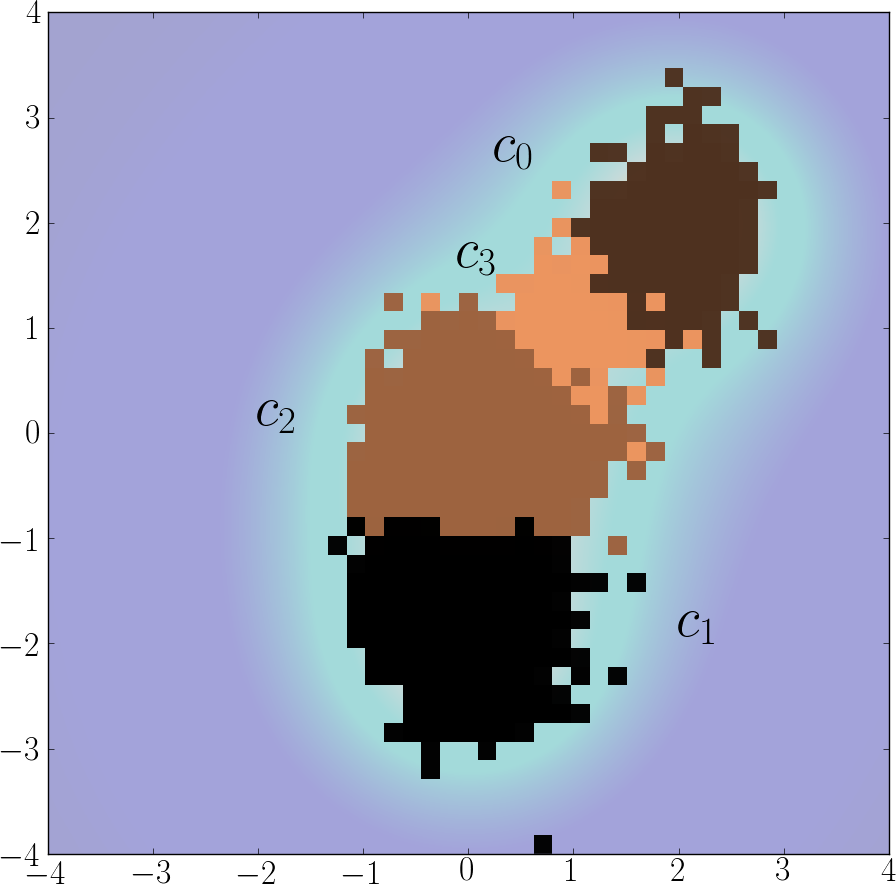
\includegraphics[width=.5\textwidth]{supplement/smooth_potential_cluster/pictures/cluster_locations.png}
    \end{tabular}
  \end{center}
  \caption{ Clusters found by partitioning the eigenflows of the FLW trajectory (Equation \ref{eq:FLW_force_eq}). Here $c_i(n)$ denotes the i\textsuperscript{th} cluster with $n$ conformational states in it. The original potential is overlaid. The algorithm found all three potential minima and identified a section as a crossing barrier.}
  \label{fig:clustering_smooth_map_cluster_loc}
\end{figure}
%
\begin{figure}[tb]
  \begin{center} \begin{tabular}{c c}
      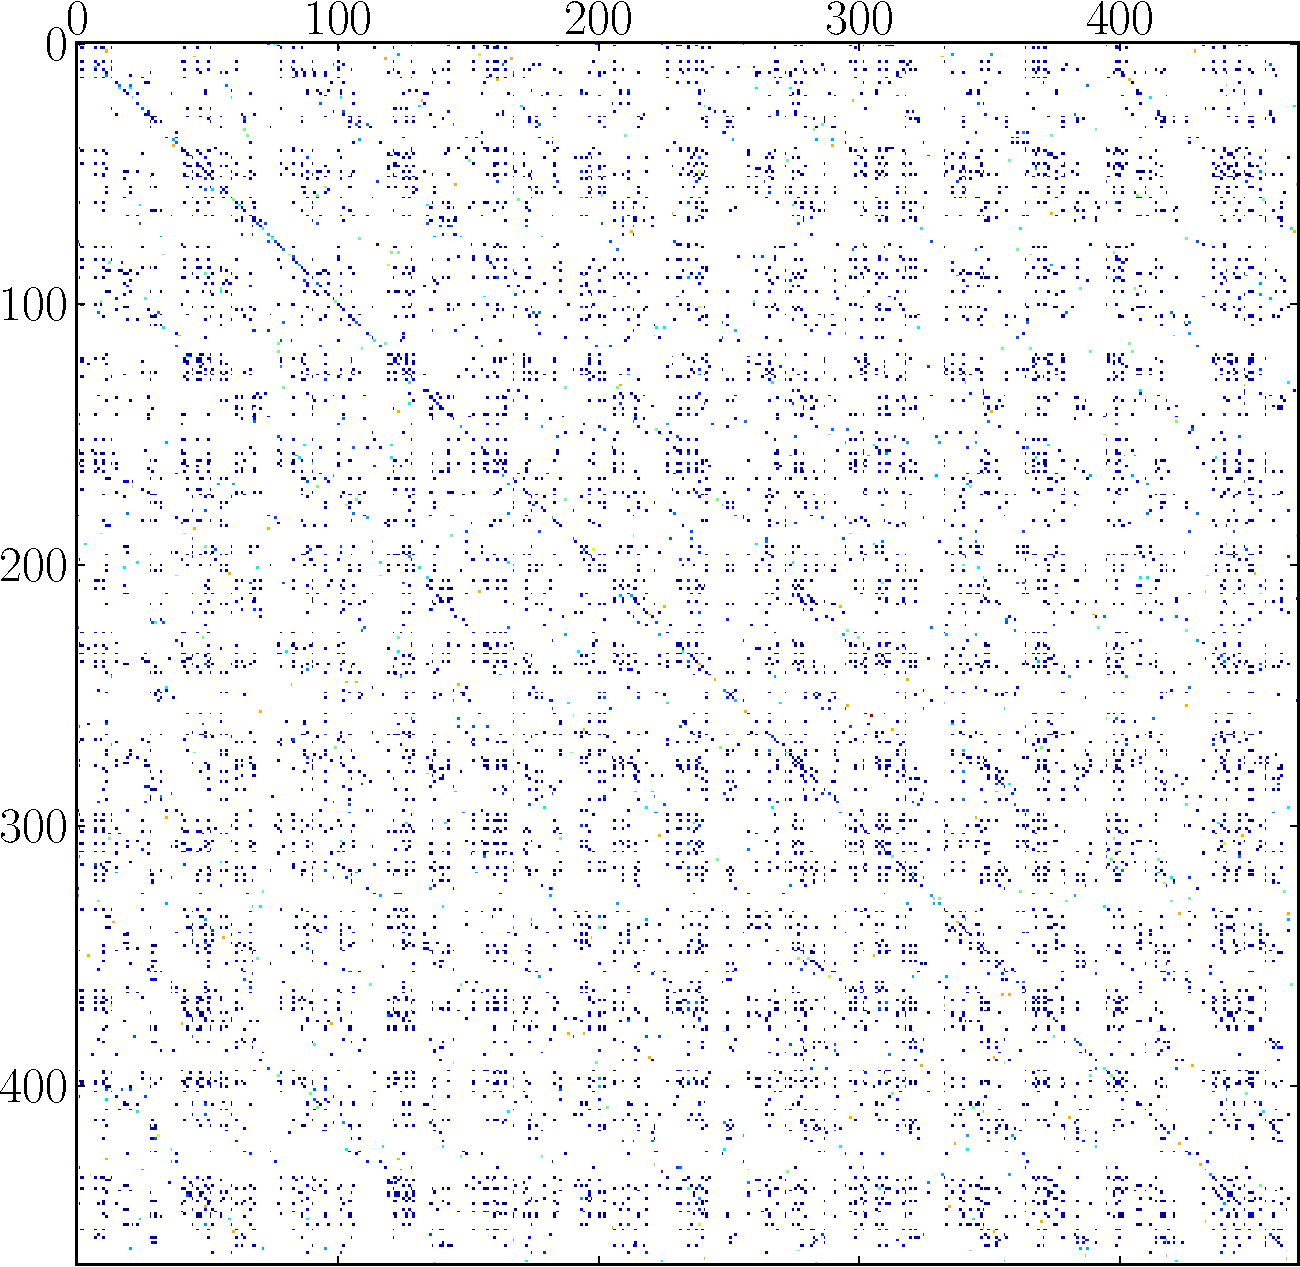
\includegraphics[width=.35\textwidth]{supplement/smooth_potential_cluster/pictures/markov_matrix_unpermuted.pdf}
      &
      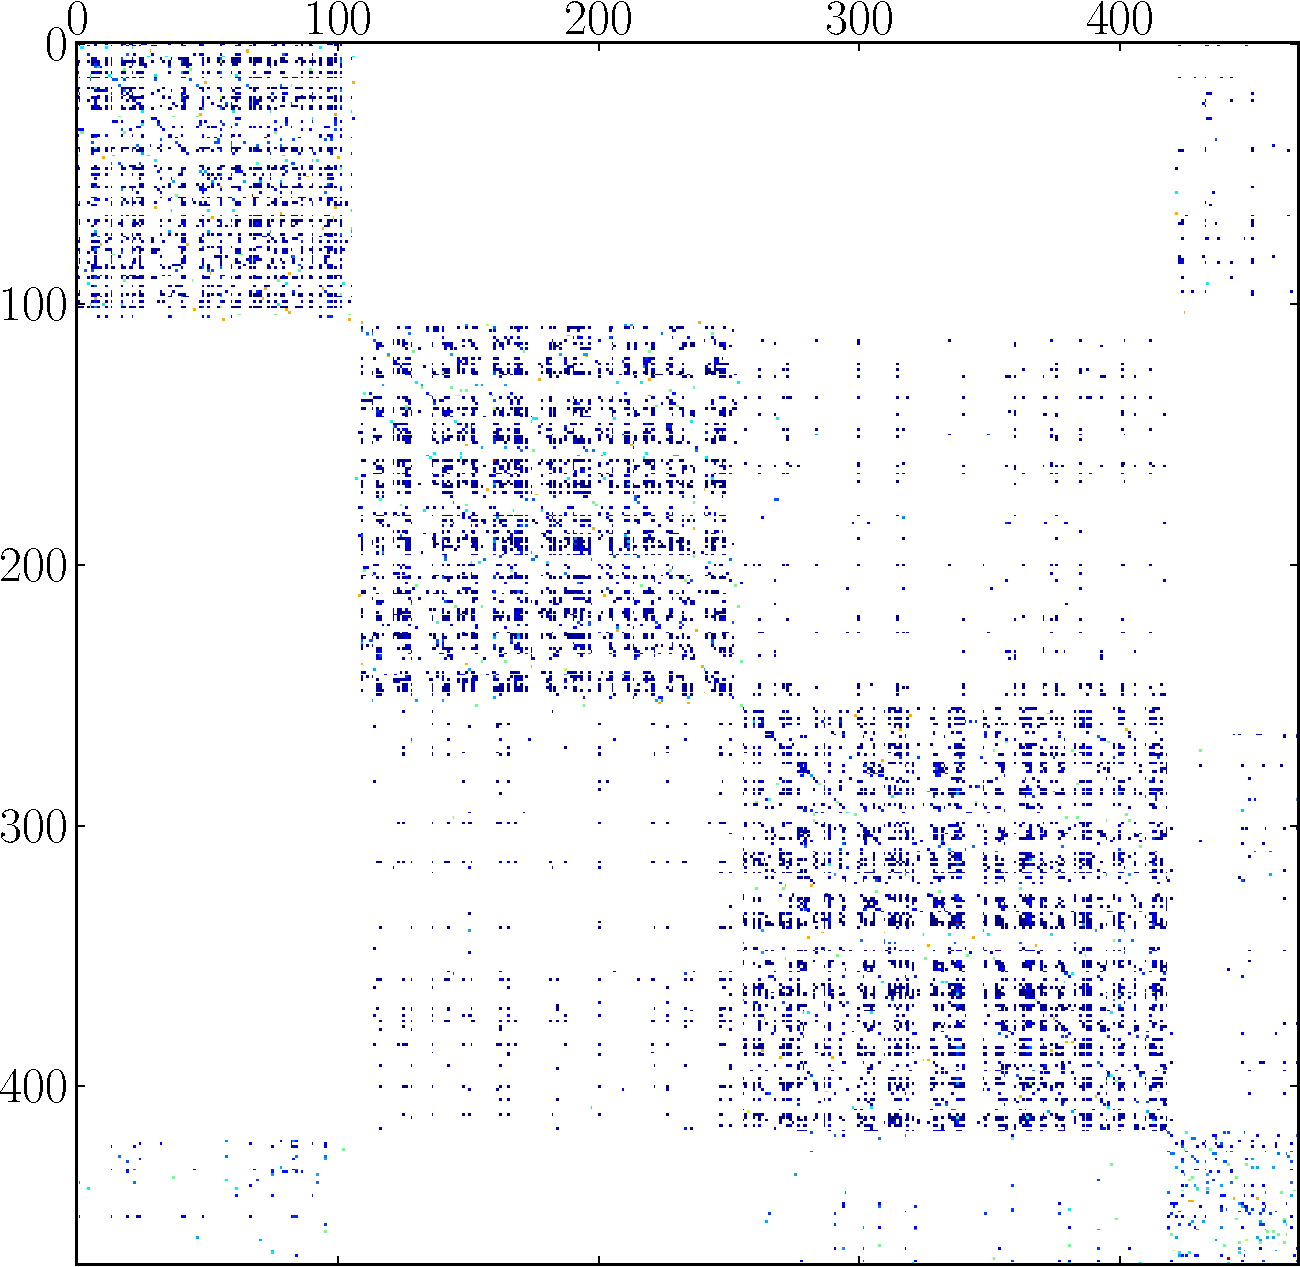
\includegraphics[width=.35\textwidth]{supplement/smooth_potential_cluster/pictures/markov_matrix_permuted.pdf}
  \end{tabular} \end{center}
  \caption{Markov transition matrix for the FLW system. The left matrix shows the states in the original, unsorted form. On the right the states have been permuted such that the states that belong to the same cluster are in adjacent rows. The block diagonal structure is clearly evident. }
  \label{fig:clustering_smooth_map_markov_permutes}
\end{figure}
%

To reduce the degrees of freedom of the system, we suggest a new kinetic pathway. With the above choice of $\phi$, all clusters have physical significance. Clusters $c_0$, $c_1$, and $c_2$ are the local minima while cluster $c_3$ is a barrier. Our model should reflect the kinetics of these four macrostates. We first computed the macrostate kinetic matrix $\B{S}$ from Equation \ref{eq:macrostate_cluster_matrix} by solving for the quasi-steady-state flows. This matrix was converted into  a rate transition matrix by the relation\footnote{
While one can compute the logarithm of a matrix, there are issues such as  embeddability and uniqueness that do not occur in the matrix exponential. Matrix $\B{A}$ is said to be embeddable if there exists a matrix $\B{B}$ such that $\B{A} = \exp(\B{B})$ and $\exp(t \B{B})$ is Markov for all $t \ge 0$. This is equivalent to taking a snapshot of an autonomous finite state Markov process that evolves continuously in time.\cite{davies_embeddable_2010} In addition, the matrix logarithm is not necessary unique. If the matrix is diagonalizable and the spectrum of eigenvalues are all strictly greater than zero, than the logarithm is unique and is given by $\log \B{A} = \B{V} \log (\B{\Gamma}) \B{V}^{-1}$. This is the Schur decomposition where the logarithm is applied to the diagonal matrix of eigenvalues. For the FLW walk, the matrix $\B{S}$ satisfied both constraints, hence the rate matrix obtained was unique.
} $t \B{W} = \log \B{S}$ giving
%
\begin{equation}
  t \B{W}_\text{reduced} = 10^{-4}
  \begin{bmatrix}
    -29  &  &  & 29 \\
    & -61 & 61 &  \\
    & 37 & -41 & 4 \\
    3181 &         & 1198 & -4377 \\
  \end{bmatrix}
\end{equation}
%
For clarity, blank entries are zero. Taking the entries of this matrix, we can now propose a simple discretized linear model for the movement in the conformational space.
%
\inlinembox{Macrostate model for FLW\vspace{.5em}}{\TIKZFLWmacrostates}
%
The macrostate characterization is complete. A new reaction coordinate for the system is suggested by this model, one that moves along the average coordinates for each macrostate. Since the macrostates are only approximations deduced from trajectories, their primary use is a categorical tool. One can also estimate first-crossing times and other kinetic predictions using various classical reaction-rate theories.\cite{haenggi_reaction-rate_1990} 

\FloatBarrier

%----------------------------------------------------------------------------------------------------------------------------

\section{Folding Pathway of a Beta-Hairpin}
%
For our second example illustrating an application of the MSC algorithm, we choose a system where the evaluation of the macrostates is not as straightforward as the FLW. Here the microstates are the various conformations of a simple lattice peptide. For a peptide, coarse-graining of the conformational space is usually achieved by various reaction coordinates such as fraction of native contacts or radius of gyration. These are selected with an \emph{a posteriori} knowledge of the physical and relevant coordinates. Here we profess ignorance of the system to see if the MSC algorithm can help determine a proper reaction coordinate. 

The general properties and behavior of lattice peptides have been detailed in the previous chapters (\cf Section \ref{sec:methods}). The peptide in our current study is constructed such that it displays both an interesting folding pathway and is a reasonable approximation to the known folding properties of a ten residue $\beta$-hairpin. Each of the ten residues has a property $r_i \in \braces{\chem{H}, \chem{P}, \chem{C_+}, \chem{C_-}, \chem{N} }$ in a \chem{H P C} bead-model Hamiltonian (hydrophobic, hydrophilic, charged residues) where $\chem{N}$ is a neutral non-interacting residue. Two residues in contact on the lattice contribute to the Hamiltonian
%
\begin{align}
  \HAM &= \sum_{i} \sum_{j>i+3} \delta(v_i,v_j) \paren{
    E_\chem{HP}(i,j) +  E_\chem{H H}(i,j) + E_\chem{PP}(i,j) +  E_\chem{C_+ C_-}(i,j) 
  }
\end{align}
Here $\delta(v_i, v_j)$ is $1$ if and only if residues $v_i$ and $v_j$ are nearest neighbors on the lattice. The energies $E_\chem{AB}$ are defined by an interaction strength $\epsilon_{\chem{AB}}$ and are non-zero if and only if residues $v_i$ and $v_j$ have the property $\chem{AB}$ (the ordering is unimportant). The magnitudes of the various interactions are
\begin{align}
  \epsilon_\chem{H P}      &= 0.1  \\ \notag
  \epsilon_\chem{P P}      &= -0.5 \\ \notag
  \epsilon_\chem{H H}      &= -0.6 \\ \notag
  \epsilon_\chem{C_+ C_-}  &= -1.5 
\end{align}
%
A picture of the unique native state is shown in Figure \ref{fig:betahairpin_nativestate}, with energy $-3.2$. This lattice Hamiltonian is one of the simplest $\beta$-hairpin models possible that captures the biological essence, namely:
%
\begin{itemize}
\item Favorable turn formation: One of the defining observed characteristics of the hairpin is the favorable internal energy the residues make at the turn. This is primarily due to the formation of a salt bridge. 
\item Realistic relative energetic magnitudes: The energies are chosen such that $- \epsilon_\chem{HP} < \epsilon_\chem{P P} < \epsilon_\chem{H H} < \epsilon_\chem{C_+ C_-}$.
\item Hydrophobic core: By including some unfavorable $\chem{HP}$ interactions we define a clear hydrophobic core that stabilizes at the center of the protein. In addition, this creates an enthalpic barrier to reach the unique native state if the protein misfolds.
\end{itemize}
%
\begin{figure}[tb]
  \TIKZbetahairpinNativestate
  \caption{Native state of the ten residue two-dimensional lattice $\beta$-hairpin. Residues marked with \chem{H}, \chem{P}, \chem{C+}, \chem{C-}, \chem{N} are hydrophobic, hydrophilic, charged, uncharged and neutral respectively.}
  \label{fig:betahairpin_nativestate}\end{figure}

Previously we've seen that sampling the state space can be done efficiently with Monte-Carlo techniques. In this case however, the state space is small enough to enumerate completely. Accounting for rotational and mirror-image symmetries there are only $N=714$ possible conformations of the system. The conformations are linked to each other by a move set of rigid rotations; every point on the chain was a permissible pivot to a new conformation as long as the resulting chain did not self-intersect. Since the chain length is less than $12$, it is known that rigid rotations for a two-dimensional lattice peptide provide sufficient ergodicity.\cite{chan_effects_1990} Numbering the conformations $\Xi=\{ \xi_1, \xi_2, ..., \xi_N \}$ we define an adjacency matrix $\B{A}$, where $\B{A}_{ij}=1$ if and only if conformation $\xi_j$ can be reached from conformation $\xi_i$ by exactly one rigid rotation.

We compute the transition rate from two states using both Metropolis and Glauber dynamics.\cite{glauber_time-dependent_1963} In both methods one needs to compute the energy difference $\Delta E_{ij} \equiv \HAM(\xi_j) - \HAM(\xi_i)$. For $i \neq j$ the transition rate matrix is specified by
\begin{itemize}
\item Metropolis dynamics
  \begin{equation}
    \B{W}_{ij} = \min (1, e ^{-\beta \Delta E_{ij}  }  )
    \label{eq:metro_dynamics}
  \end{equation}
\item Glauber dynamics
  \begin{equation}
    \B{W}_{ij} = \frac { e ^{-\beta \Delta E_{ij}}}  { 1 + e ^{-\beta \Delta E_{ij}} }
    \label{eq:glauber_dynamics}
  \end{equation}
\end{itemize}
For $i=j$, $\B{W}_{ii} = - \sum_{k \neq j} \B{W}_{kj}$ (see Section \ref{sec:master_equations} for additional details on the master equation formulation). We take the exponential of this matrix to get a Markovian one, $\B{M}=\exp (t \B{W})$ with $t=0.5$ and $\beta=4$. While different rates were obtained using Glauber and Metropolis dynamics, there was no discernible difference in the results of the MSC algorithm. As in the previous problem with the FLW system, we show the original and permuted Markov matrices in Figure \ref{fig:Rate_Matrix_Permutations}. The block diagonal structure can be seen for small isolated clusters, but a large majority of conformations reside in the large block. Examining the states in this cluster we see that these are the random coil states. 
\begin{figure}[tb]
  \begin{center}
    \begin{tabular}{c c}
      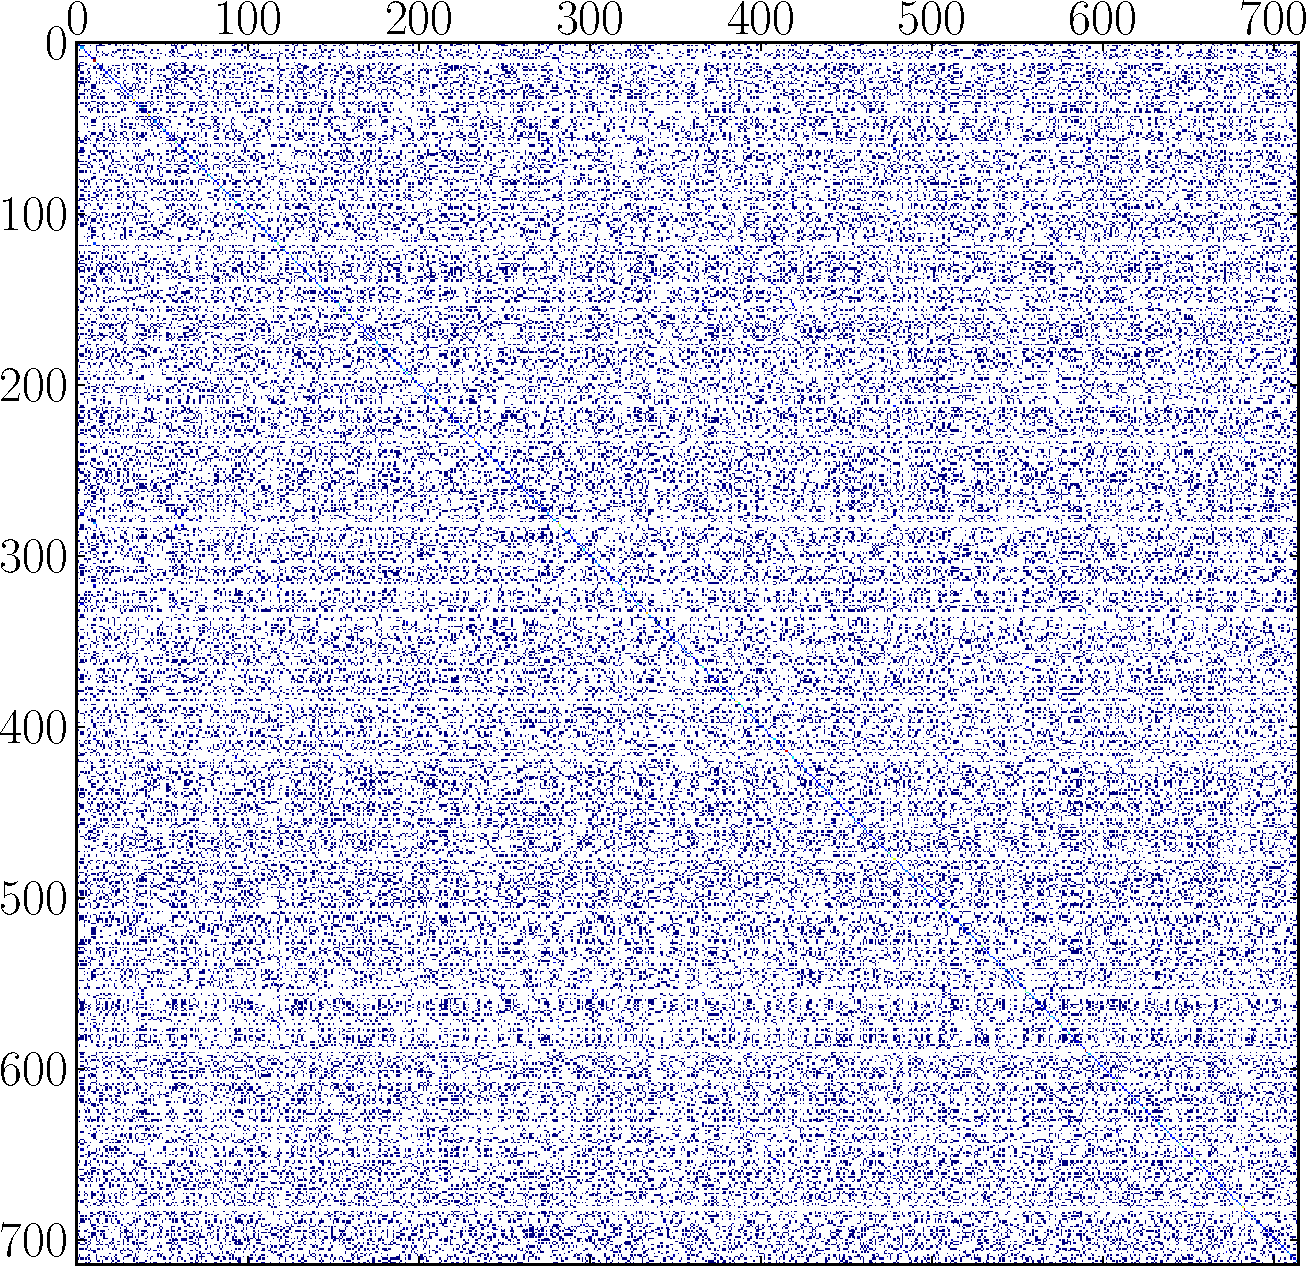
\includegraphics[width=.35\textwidth]{supplement/beta_cluster_example_2/pictures/markov_matrix_unpermuted.pdf}
      &
      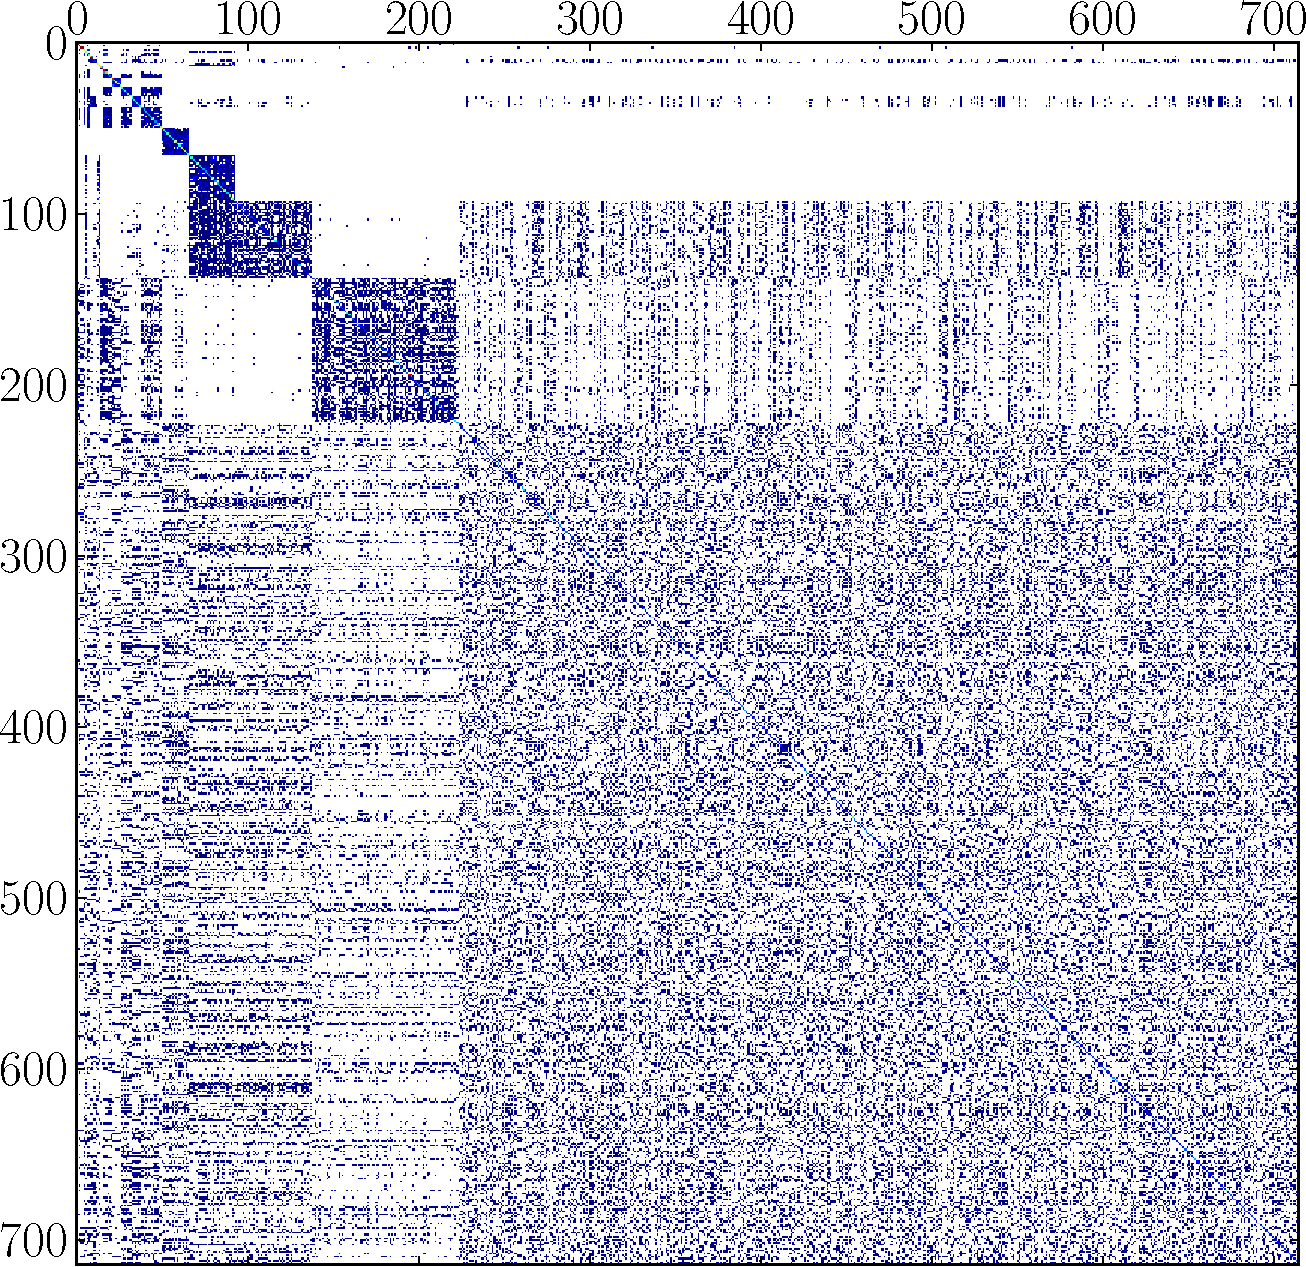
\includegraphics[width=.35\textwidth]{supplement/beta_cluster_example_2/pictures/markov_matrix_permuted.pdf}
    \end{tabular}
  \end{center}
  \caption{Markov transition matrix for the $\beta$-hairpin system using Glauber dynamics. The left matrix shows the states in the original, unsorted form where the states were enumerated by rigid rotations. On the right, the matrix has been permuted such that the states that belong to the same cluster are in adjacent rows. The block diagonal structure is clearly evident, with a large fraction of the states grouped into a single cluster. }
  \label{fig:Rate_Matrix_Permutations}
\end{figure}

\subsection{Folding Nucleation}
In this system there were $22$ identified clusters, though not all of them were physically relevant. To see why, we start the system in an initial state of the fully extended random coil $b_c$. We advance the system in time via $b_c \B{S}^t$ and plot the occupational probabilities of the clusters. In Figure \ref{fig:beta_hairpin_kinetics} we see the long-time behavior of the system. In the figure we order the clusters by the number of microstates they contain to illustrate the magnitude of the largest cluster. The ordering of the clusters is unimportant, any permutation would give the same macrostate information. This cluster $c_{21}$, contained $493$ microstates and had the initial state as one of its members. However the system quickly and cooperatively folded into two different clusters with a much smaller number of microstates. These clusters $c_{17}$ and $c_{18}$ had $16$ and $27$ microstates respectively. We identified them as intermediate states of the folding processes as they eventually decayed before reaching a final cluster $c_{11}$ with only two microstates. 
%
\begin{figure}[tb]
  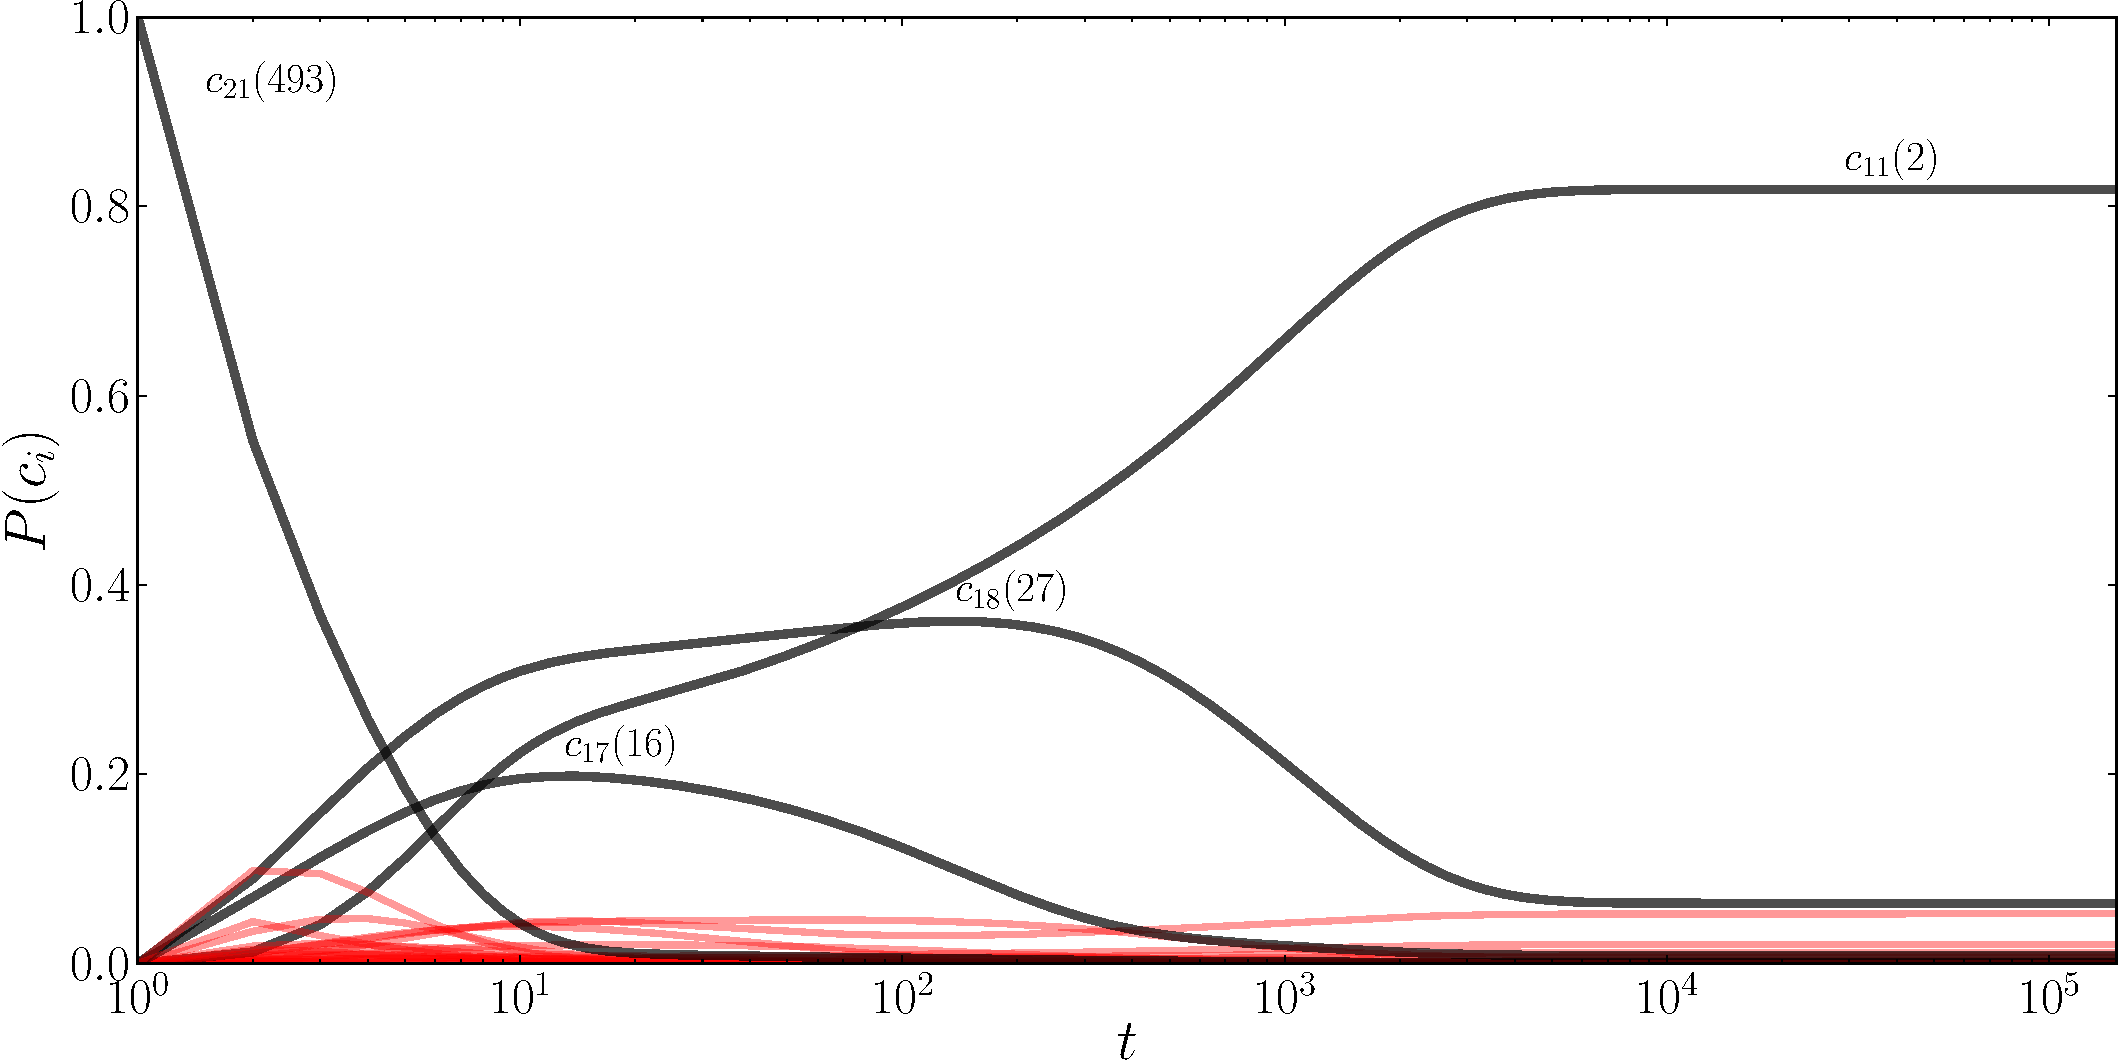
\includegraphics[width=\textwidth]{supplement/beta_cluster_example_2/pictures/kinetics_beta_cluster.pdf}
  \caption{
    Cluster kinetics for the $\beta$-hairpin over a logarithmic time axis. Starting at the completely unfolded state, the motion spans many decades before it folds in the native state. For clarity, the clusters with a significant population are labeled and shown in black. The other clusters are shown in red.
  }
  \label{fig:beta_hairpin_kinetics}
\end{figure}
%

With the interesting clusters identified, we can examine them for any shared property. The microstates are shown at different scales for visual clarity (long, narrow microstates may appear smaller than globular ones). Shown below is the final cluster $c_{11},$ clearly containing native state.
\inlineframebox{\B{Native state cluster} $c_{11}$}{
  \begin{tabular}{ c c }
    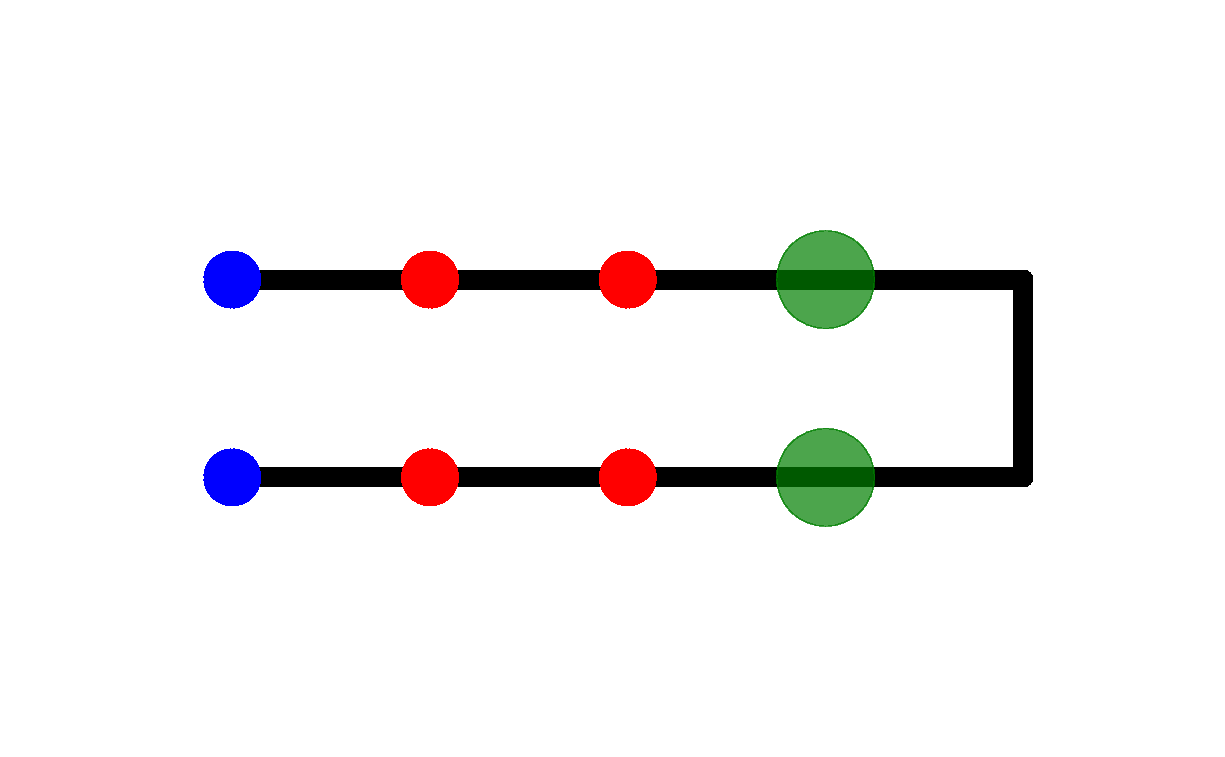
\includegraphics[width=.25\textwidth]{supplement/beta_cluster_example_2/pictures/saved_macrostates/state_cluster_shapes_0.png} 
    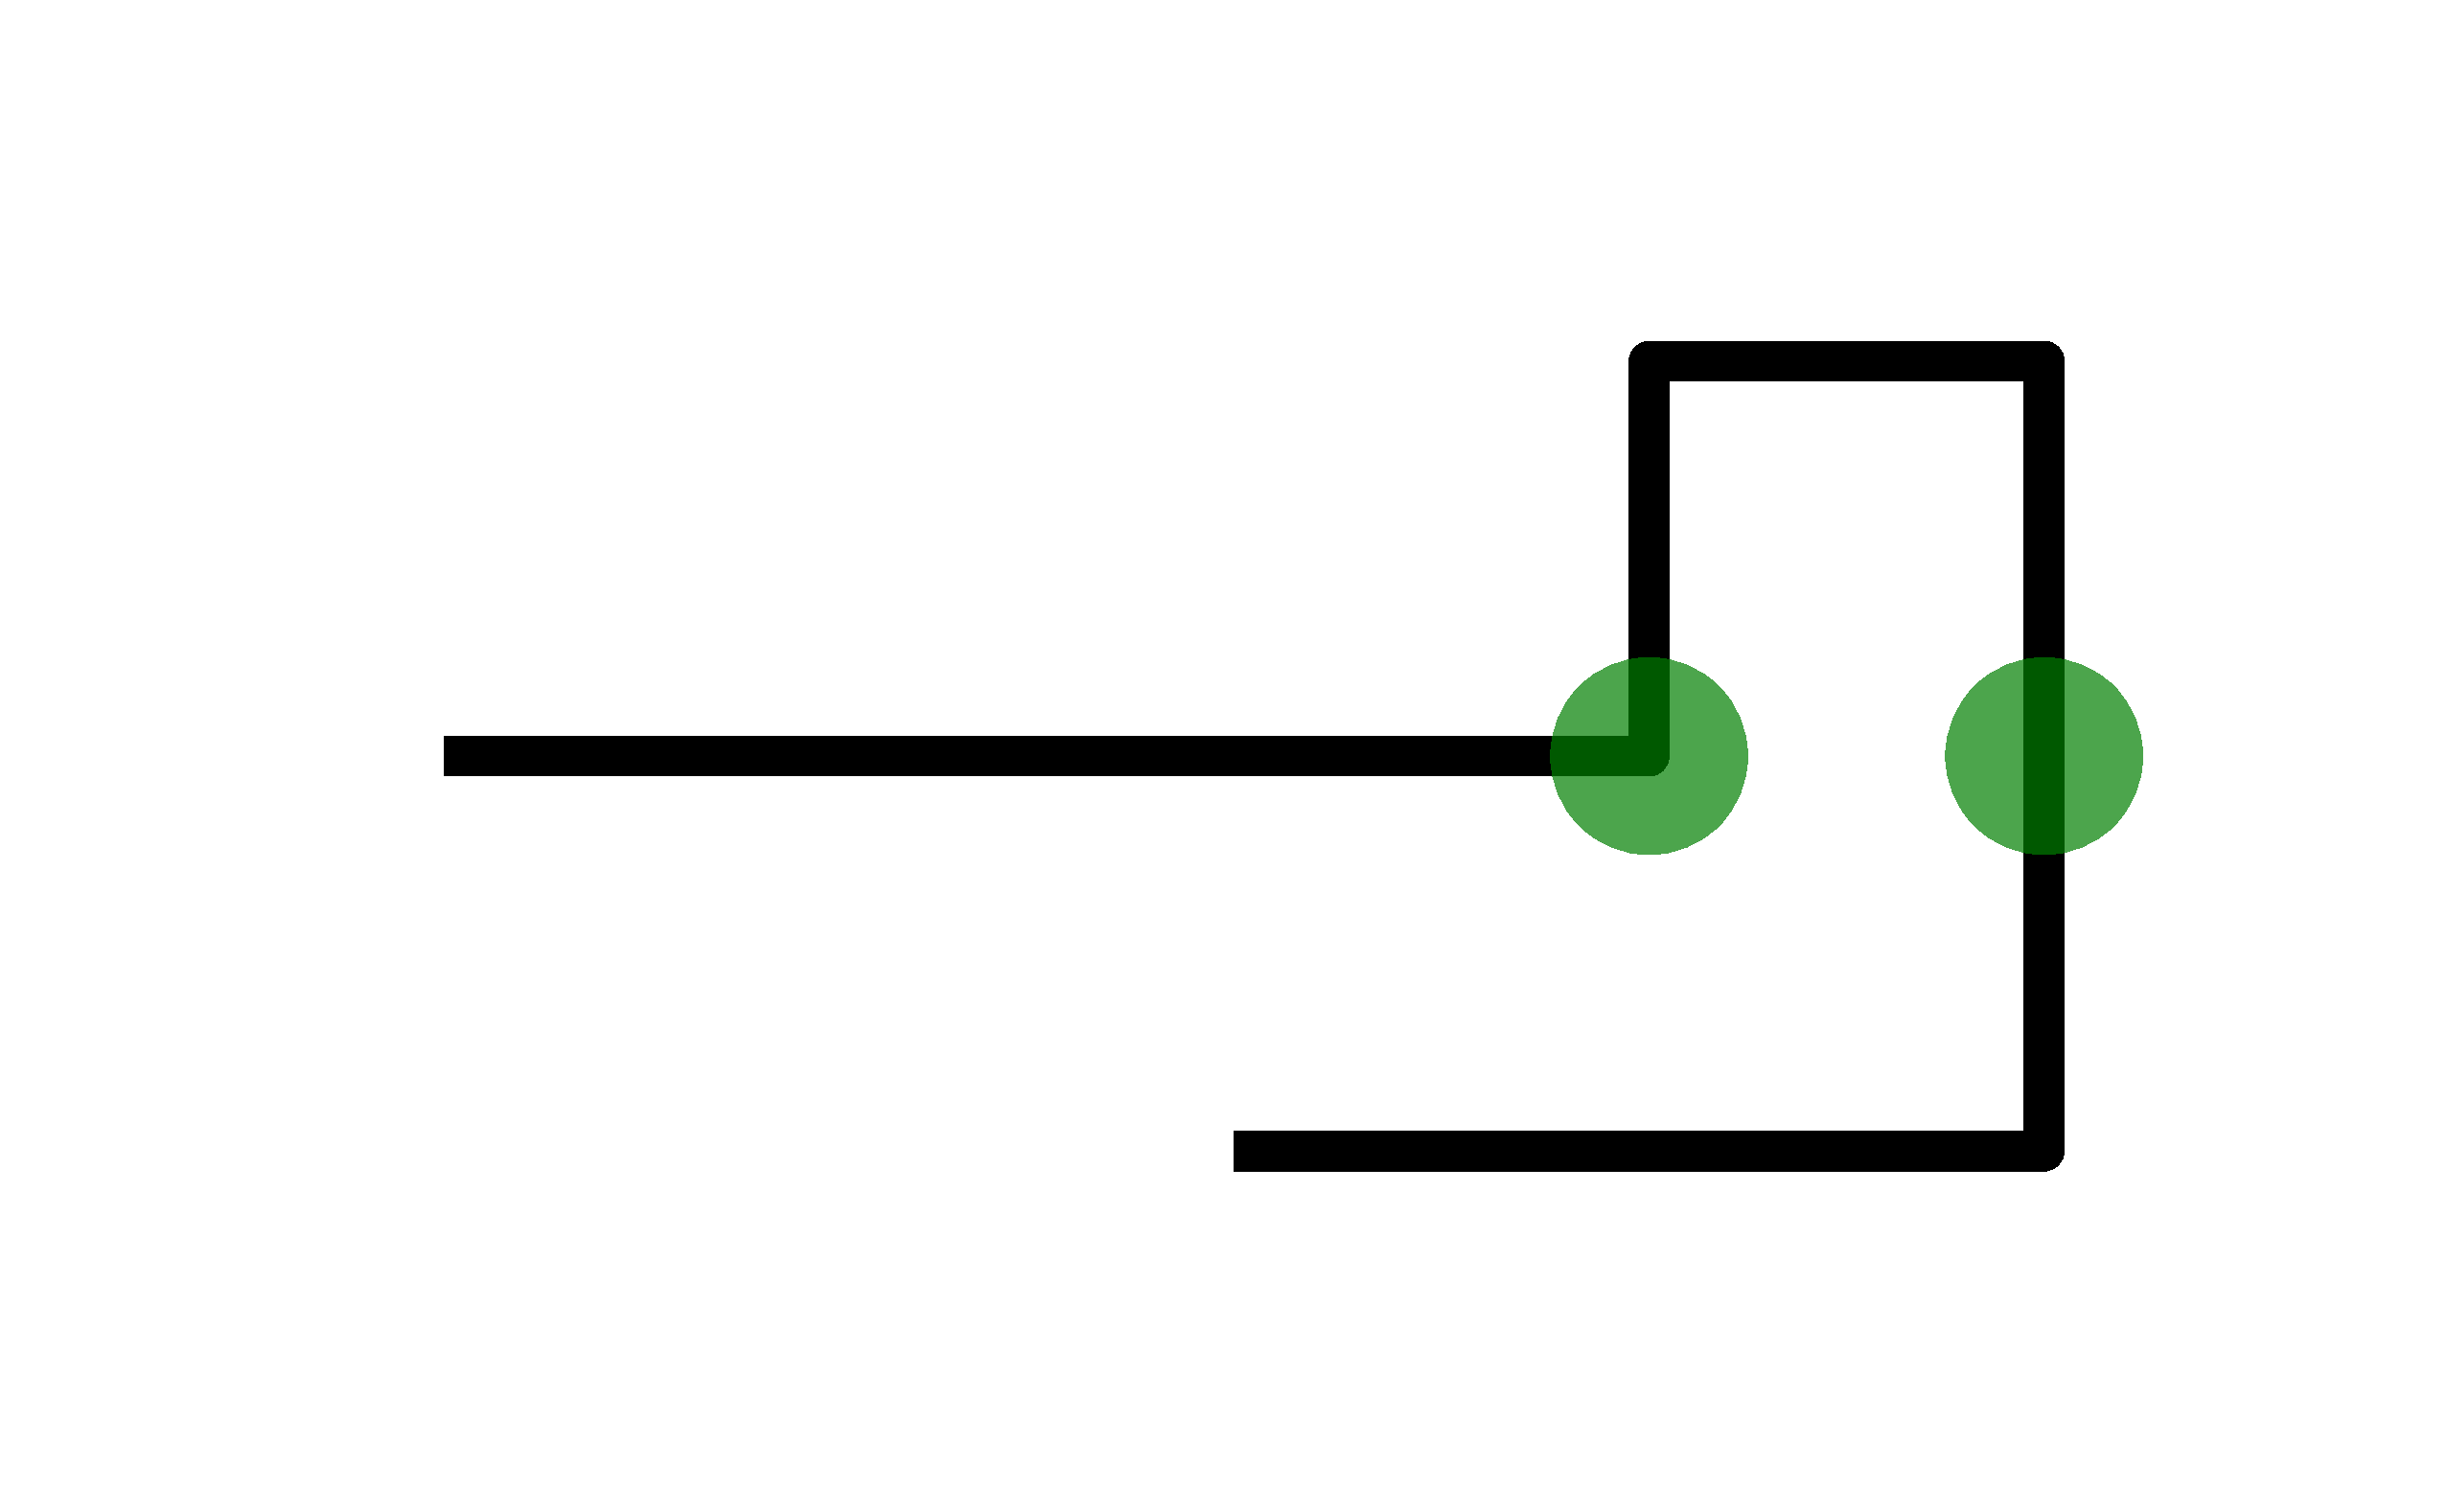
\includegraphics[width=.25\textwidth]{supplement/beta_cluster_example_2/pictures/11/state_cluster_shapes_1.pdf} 
  \end{tabular}
}
The presence of an additional microstate is not unexpected. As we saw before in the FLW walk, local minima are often associated with the same cluster.
All of the microstates in the other two intermediate clusters have one particular thing in common, the formation of the salt bridge. Listed below are six representative conformations in each of the two intermediate clusters
%
\inlineframebox{\B{Intermediate Cluster} $c_{17}$} {
  \begin{tabular}{ c c c }
    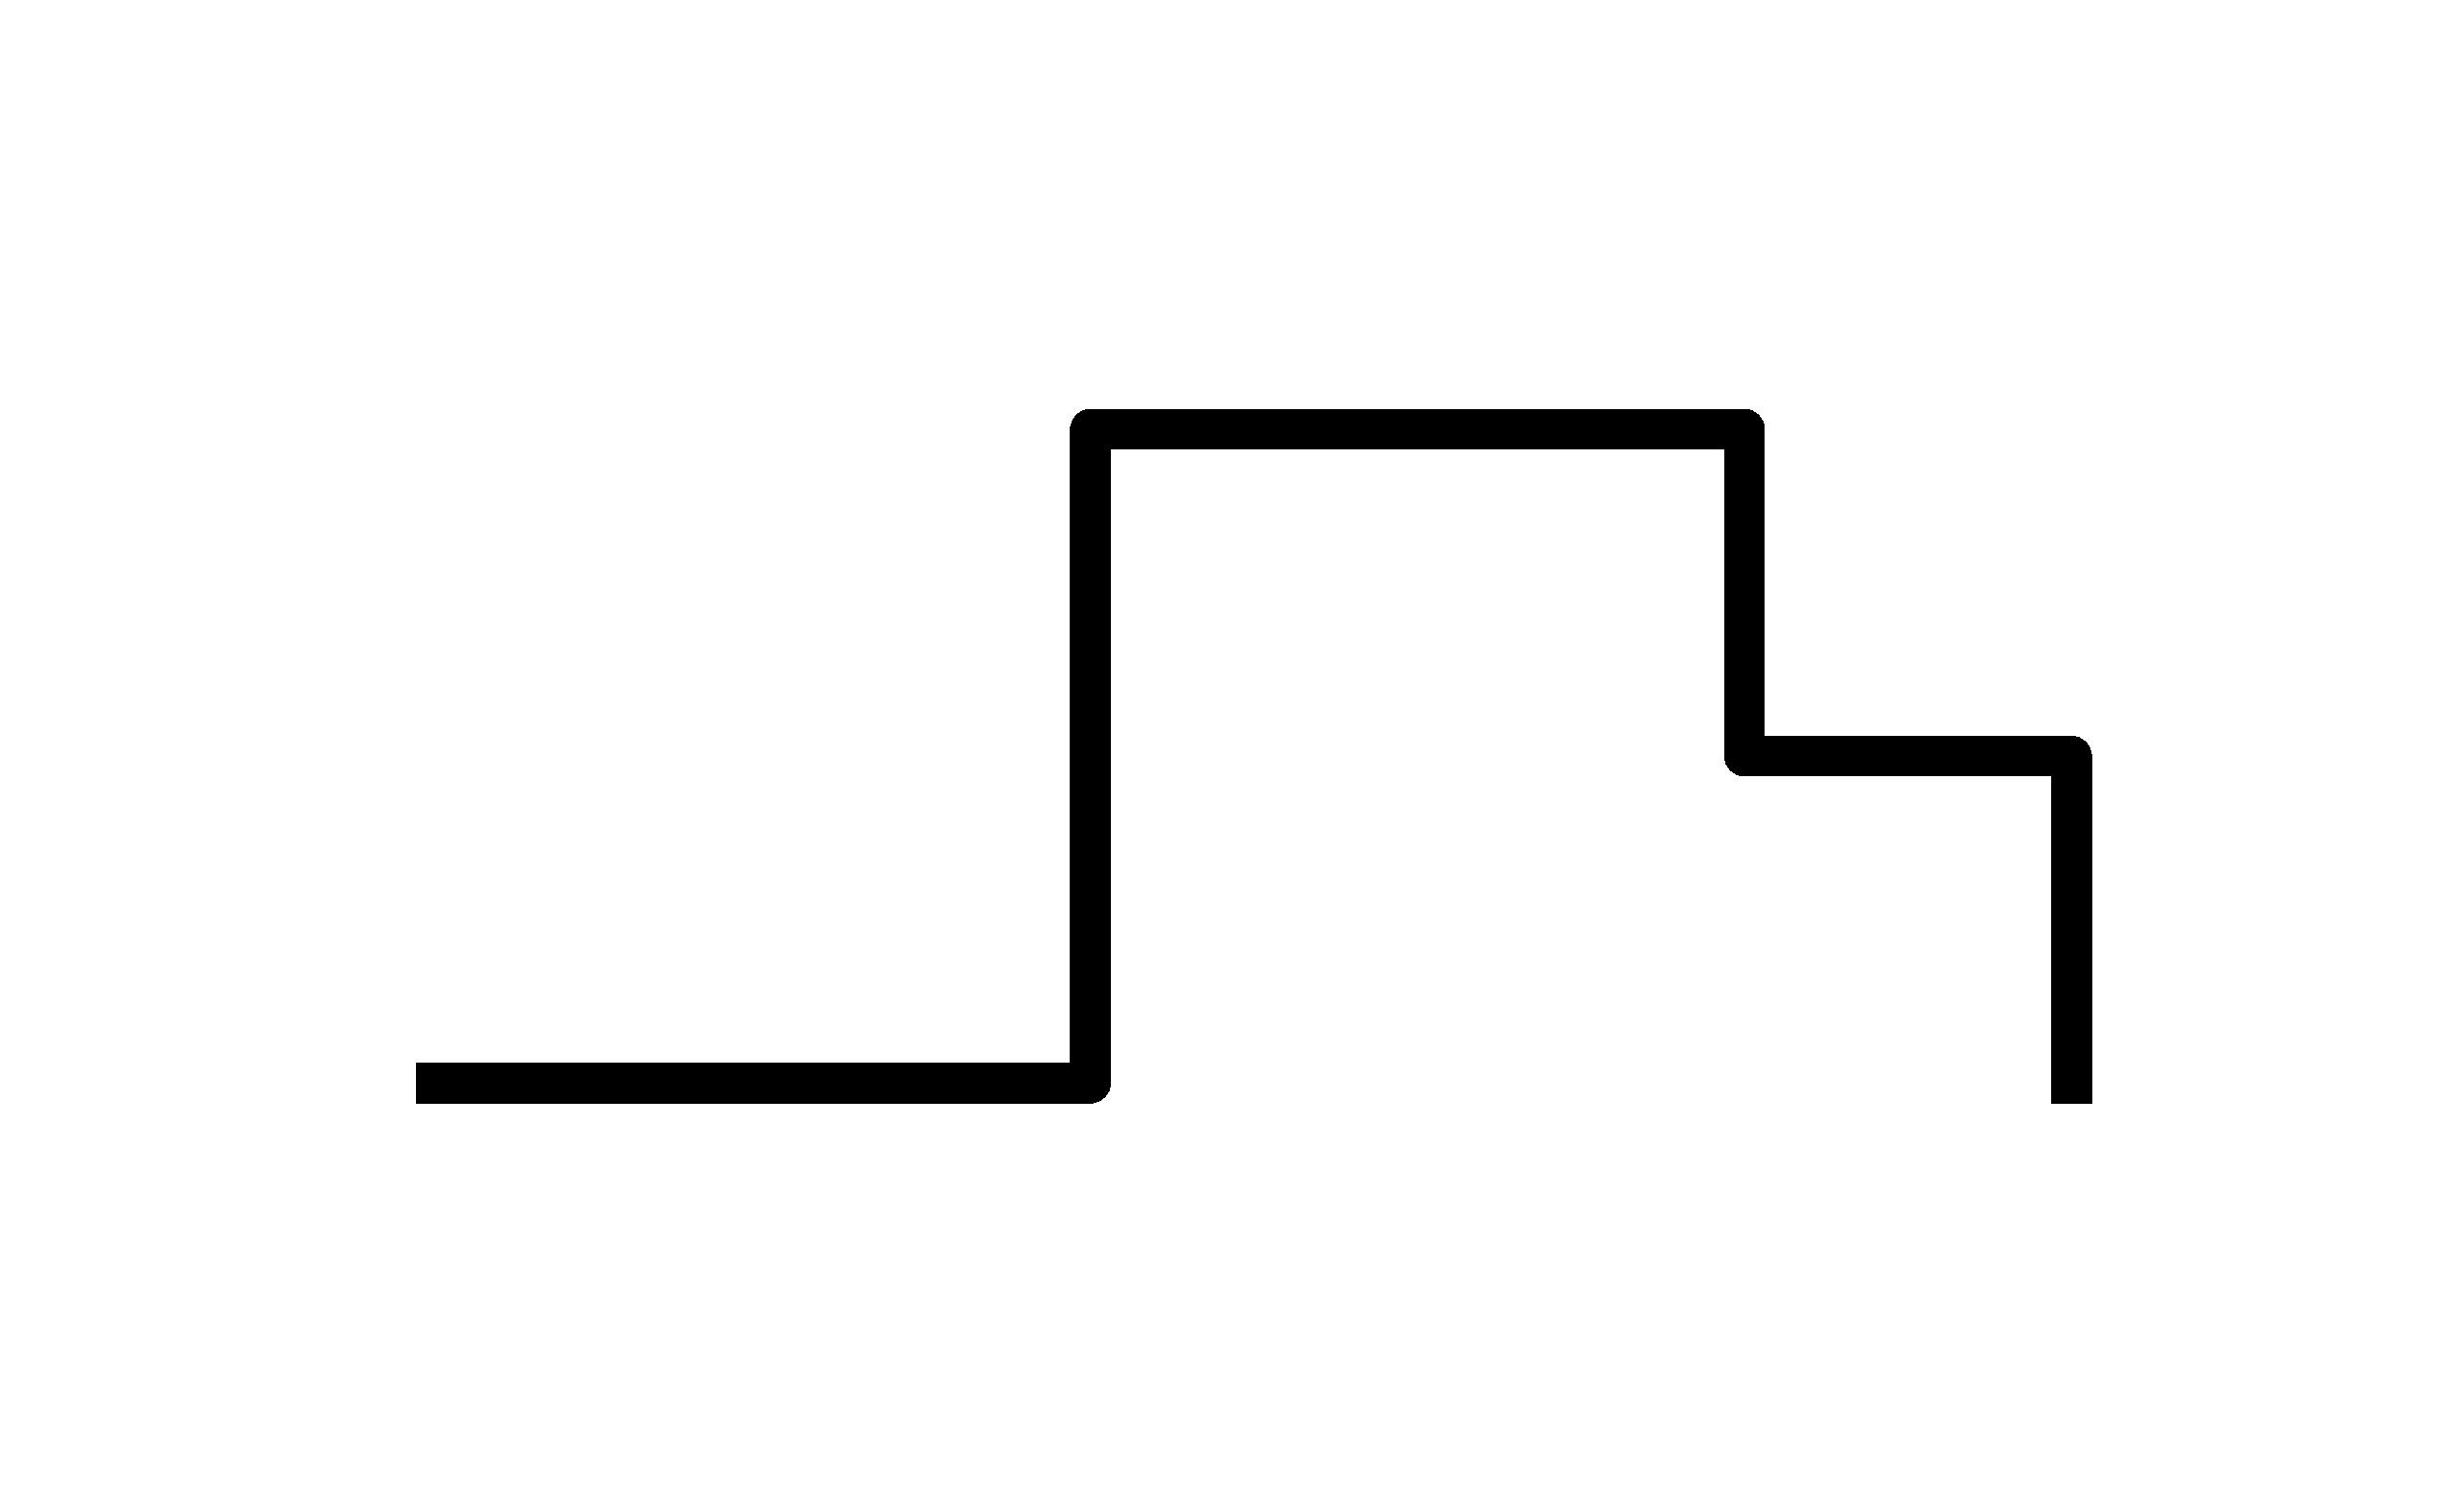
\includegraphics[width=.252\linewidth]{supplement/beta_cluster_example_2/pictures/17/state_cluster_shapes_0.pdf} &
    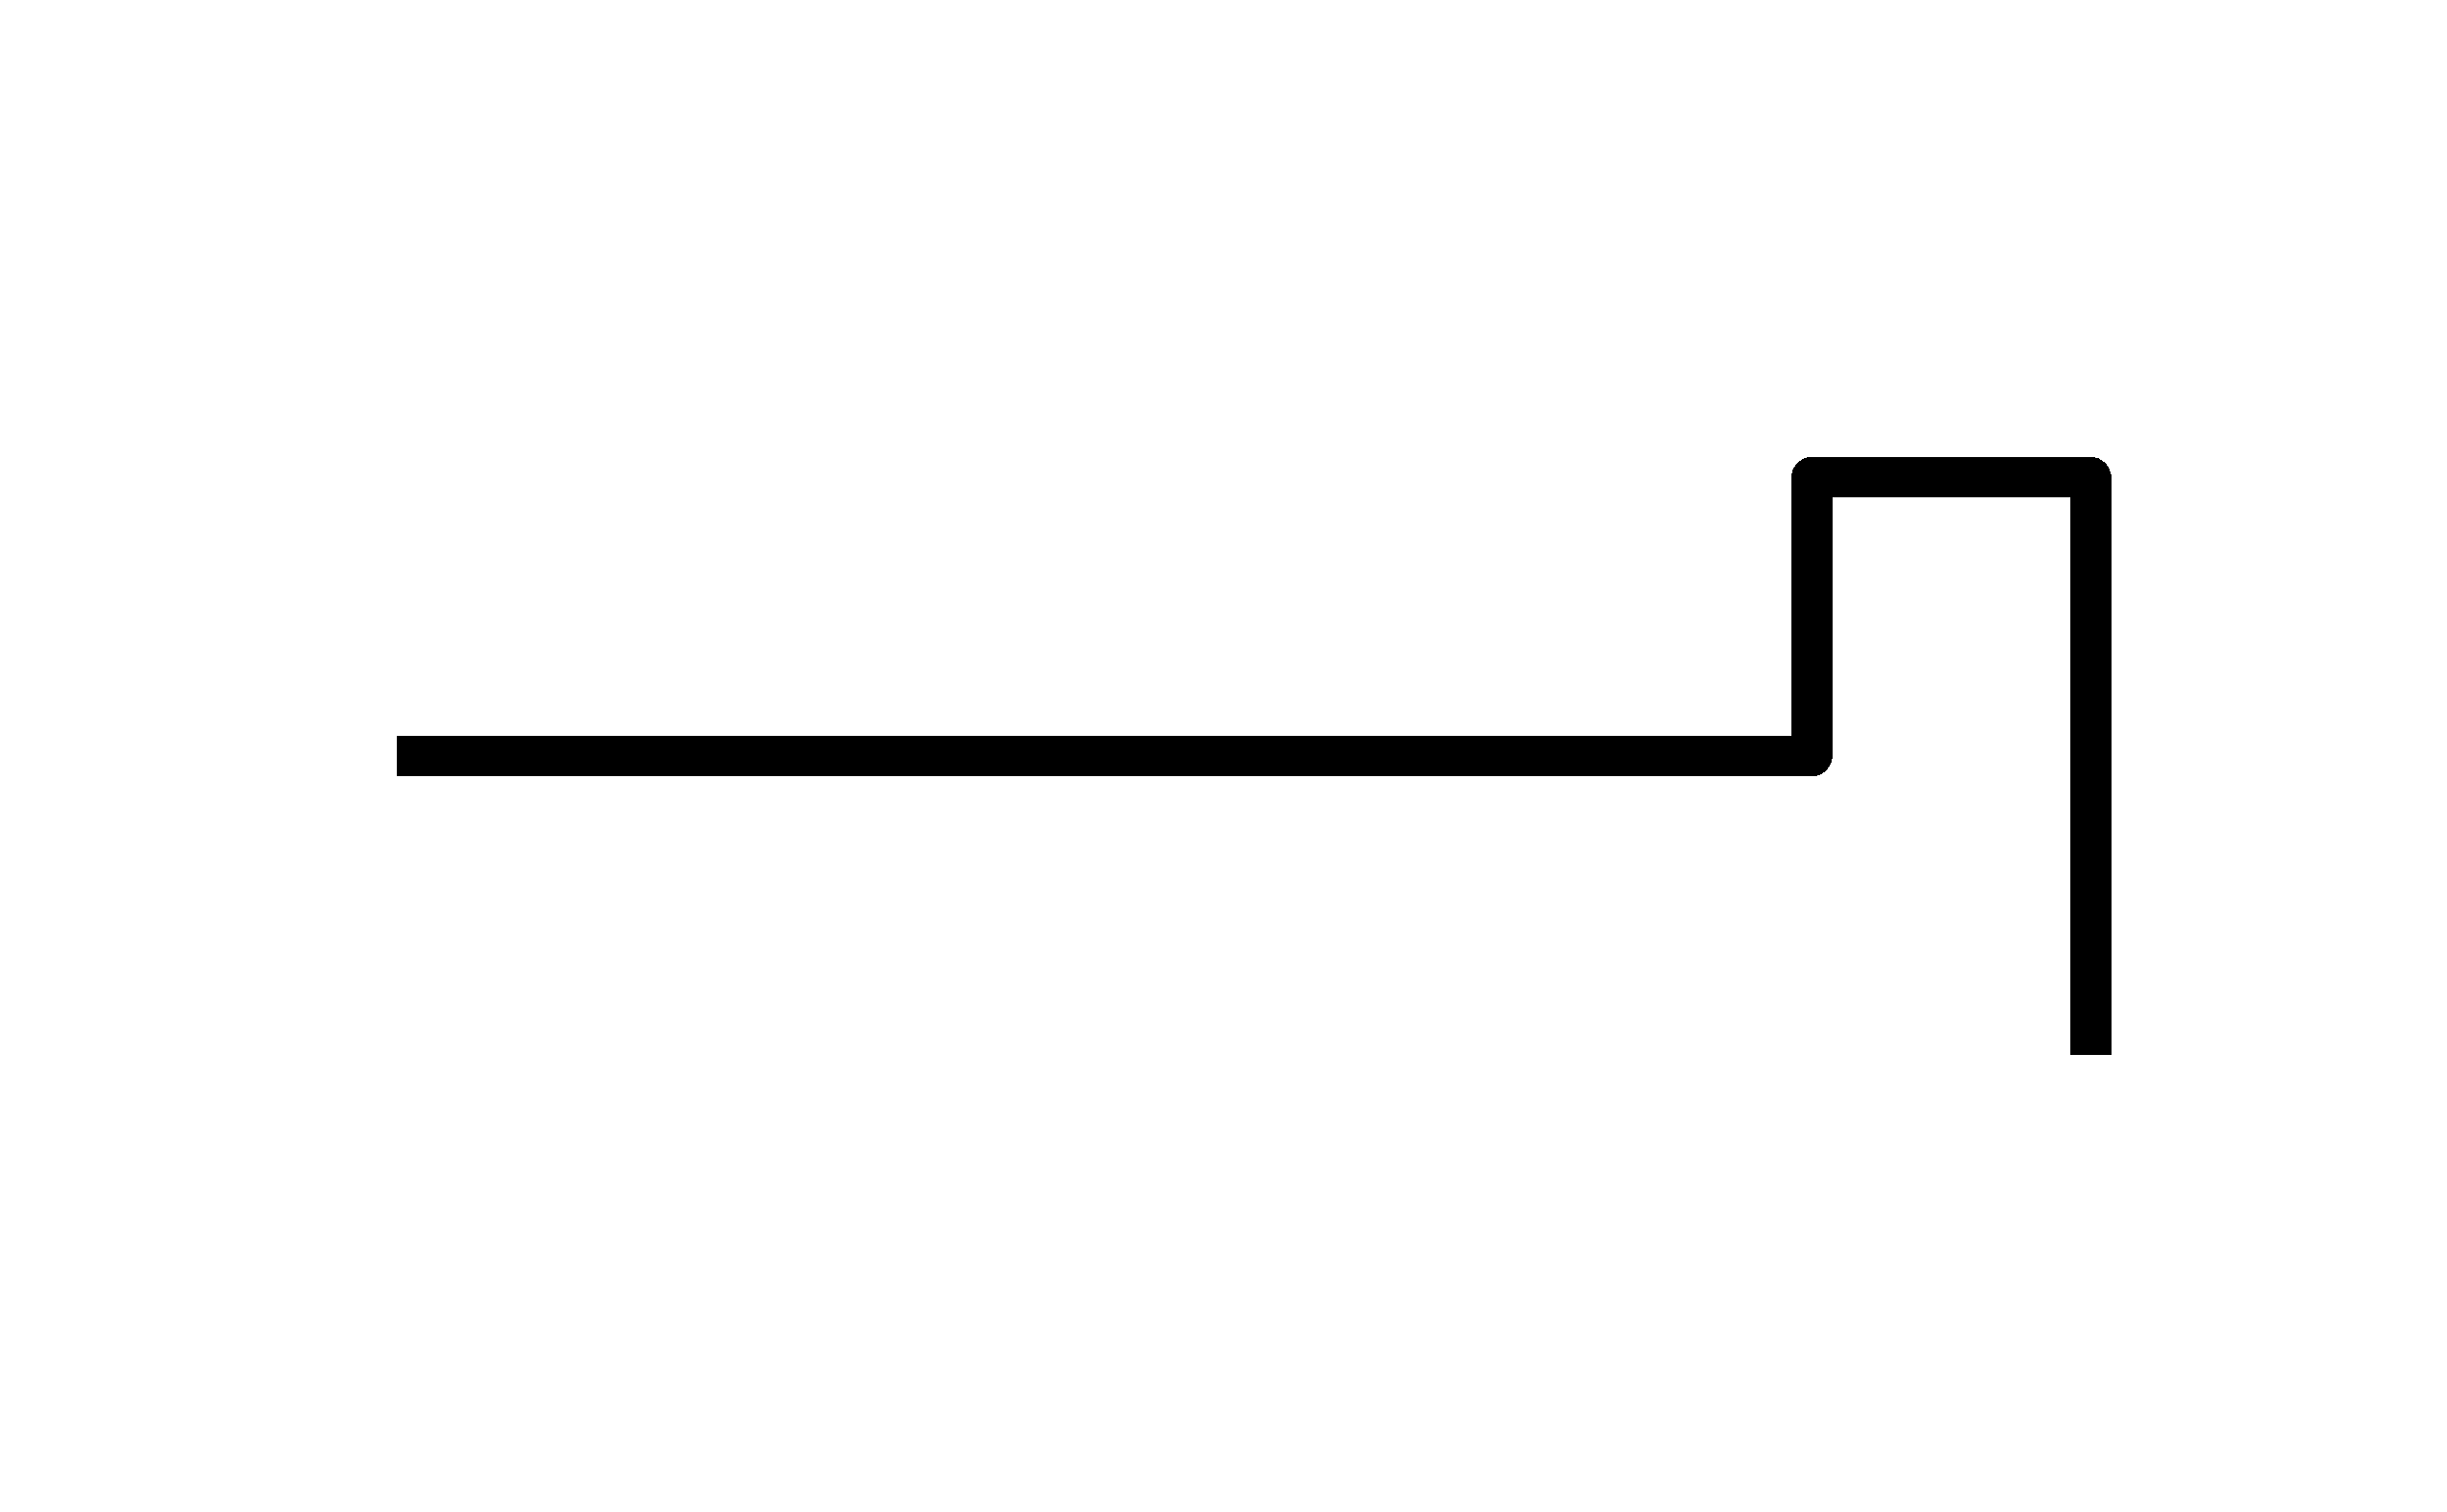
\includegraphics[width=.252\linewidth]{supplement/beta_cluster_example_2/pictures/17/state_cluster_shapes_1.pdf} & 
    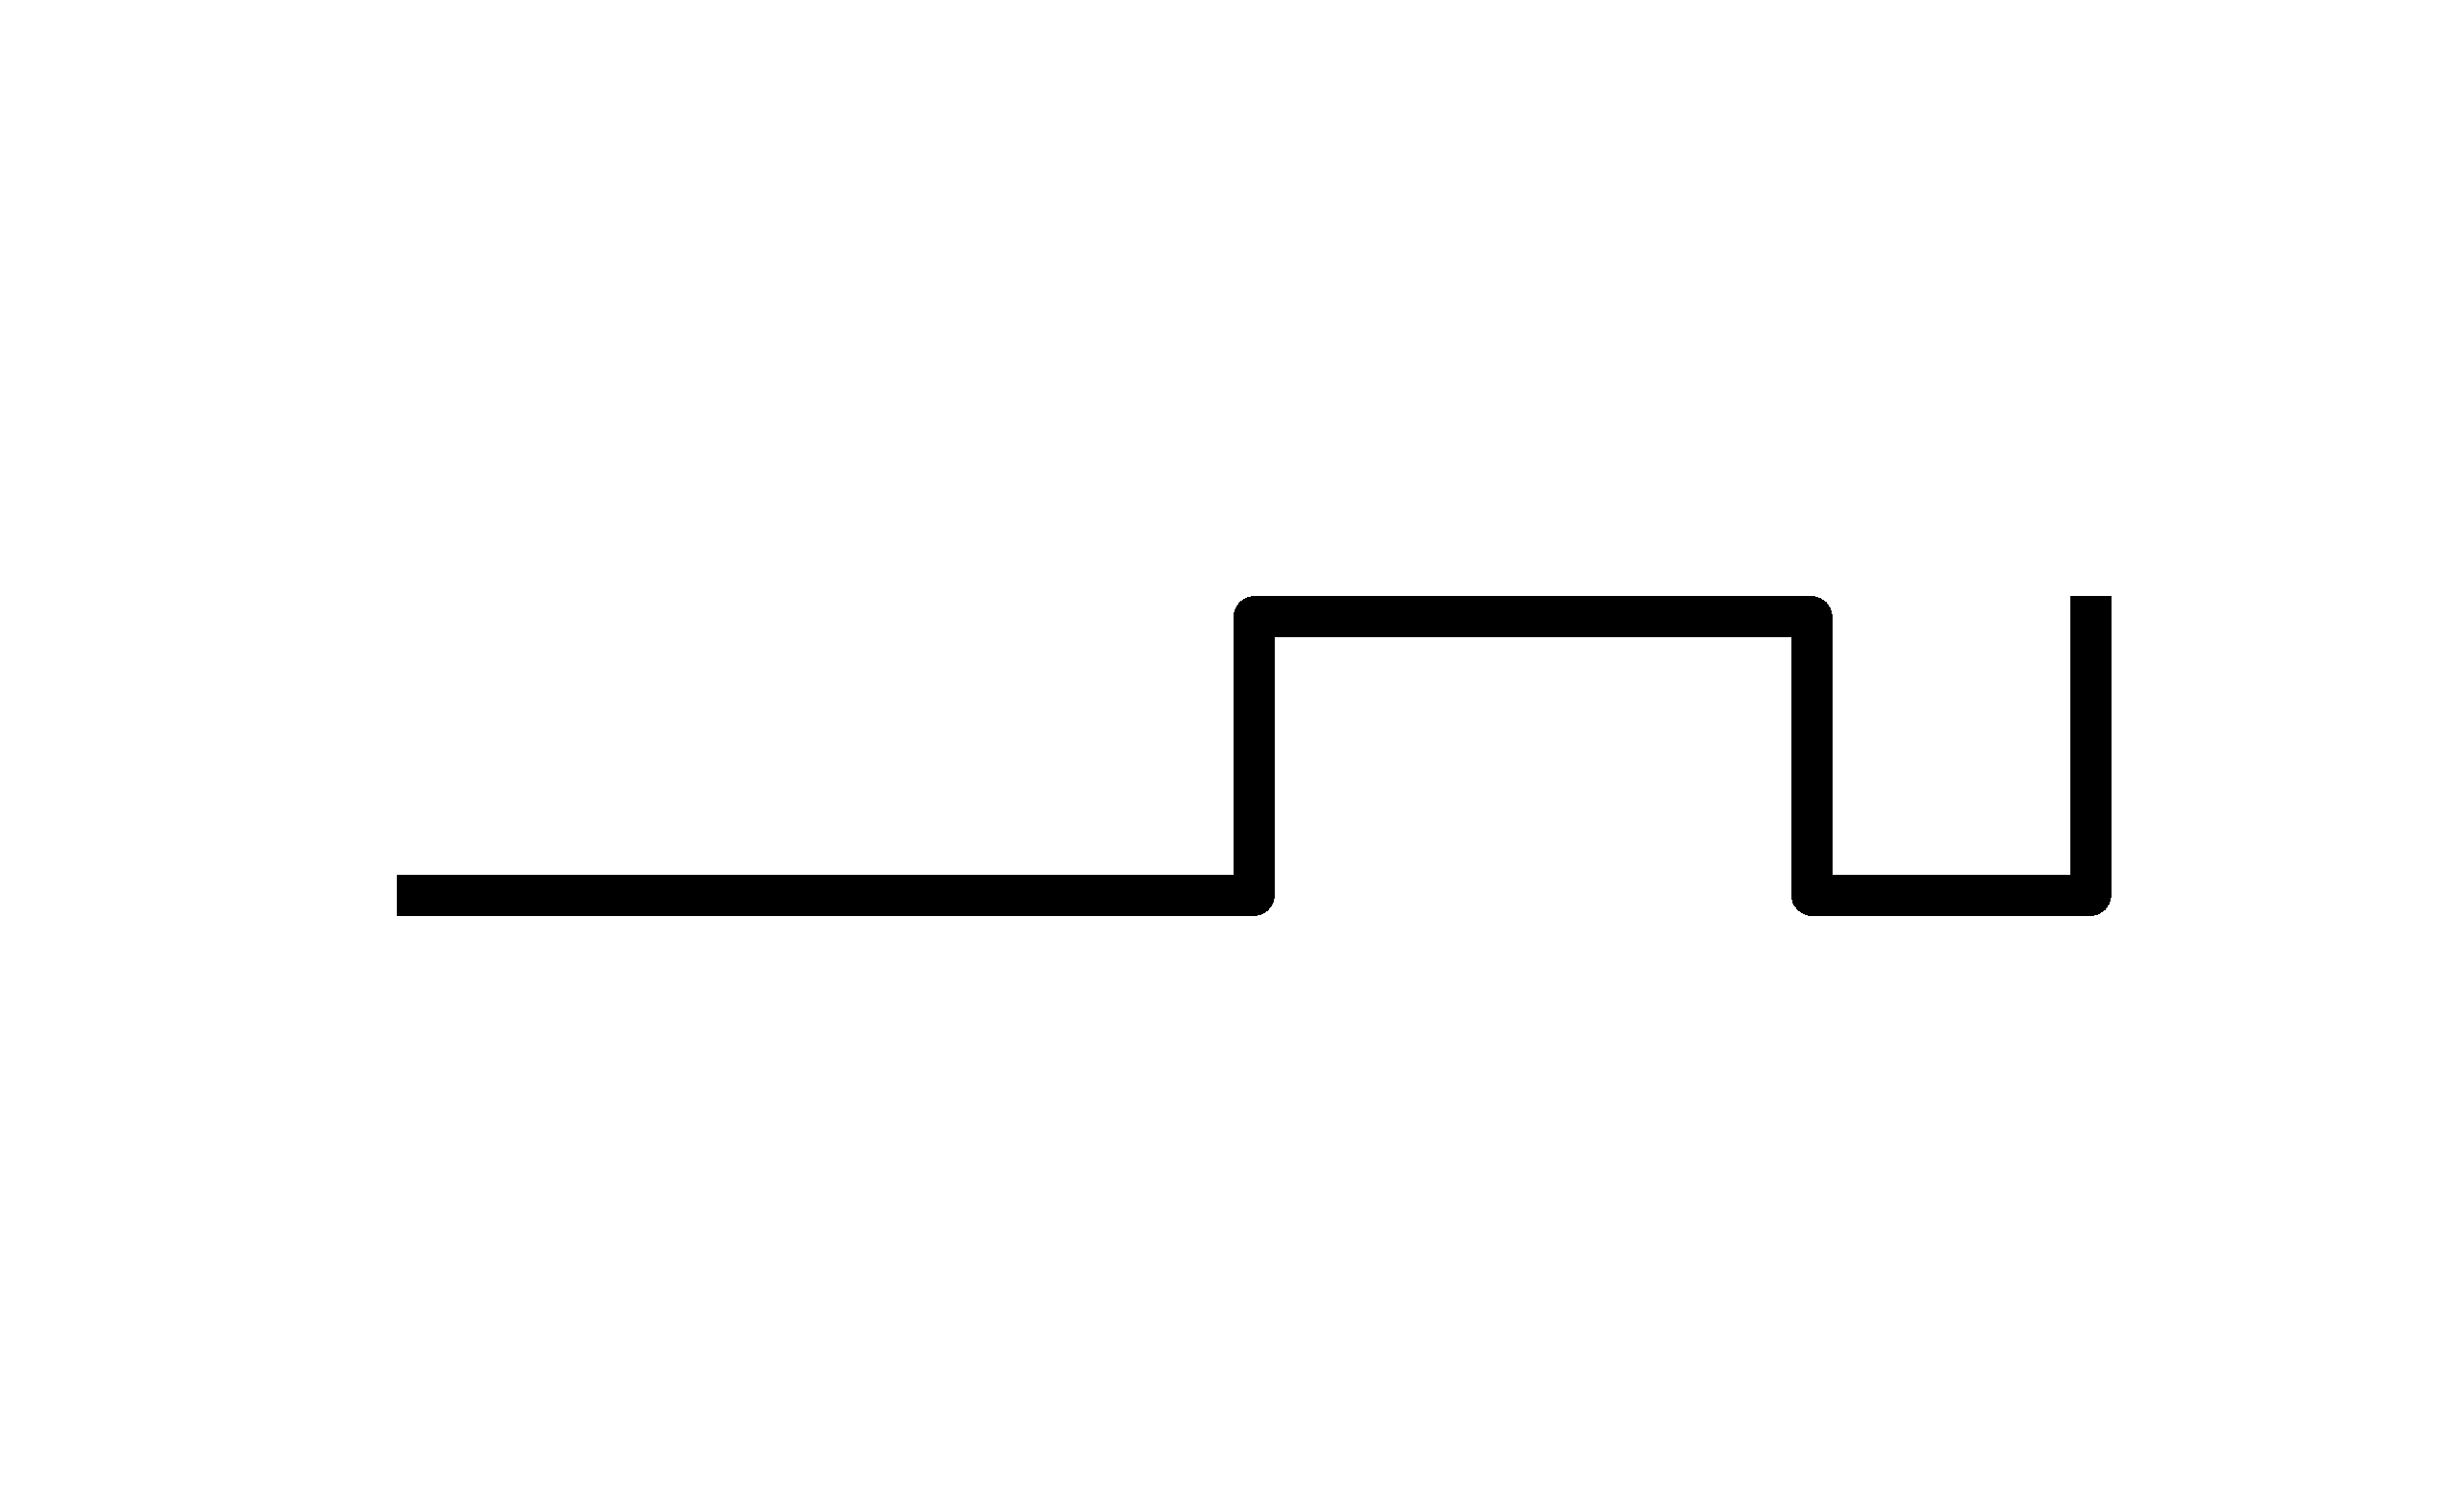
\includegraphics[width=.252\linewidth]{supplement/beta_cluster_example_2/pictures/17/state_cluster_shapes_2.pdf} \\
    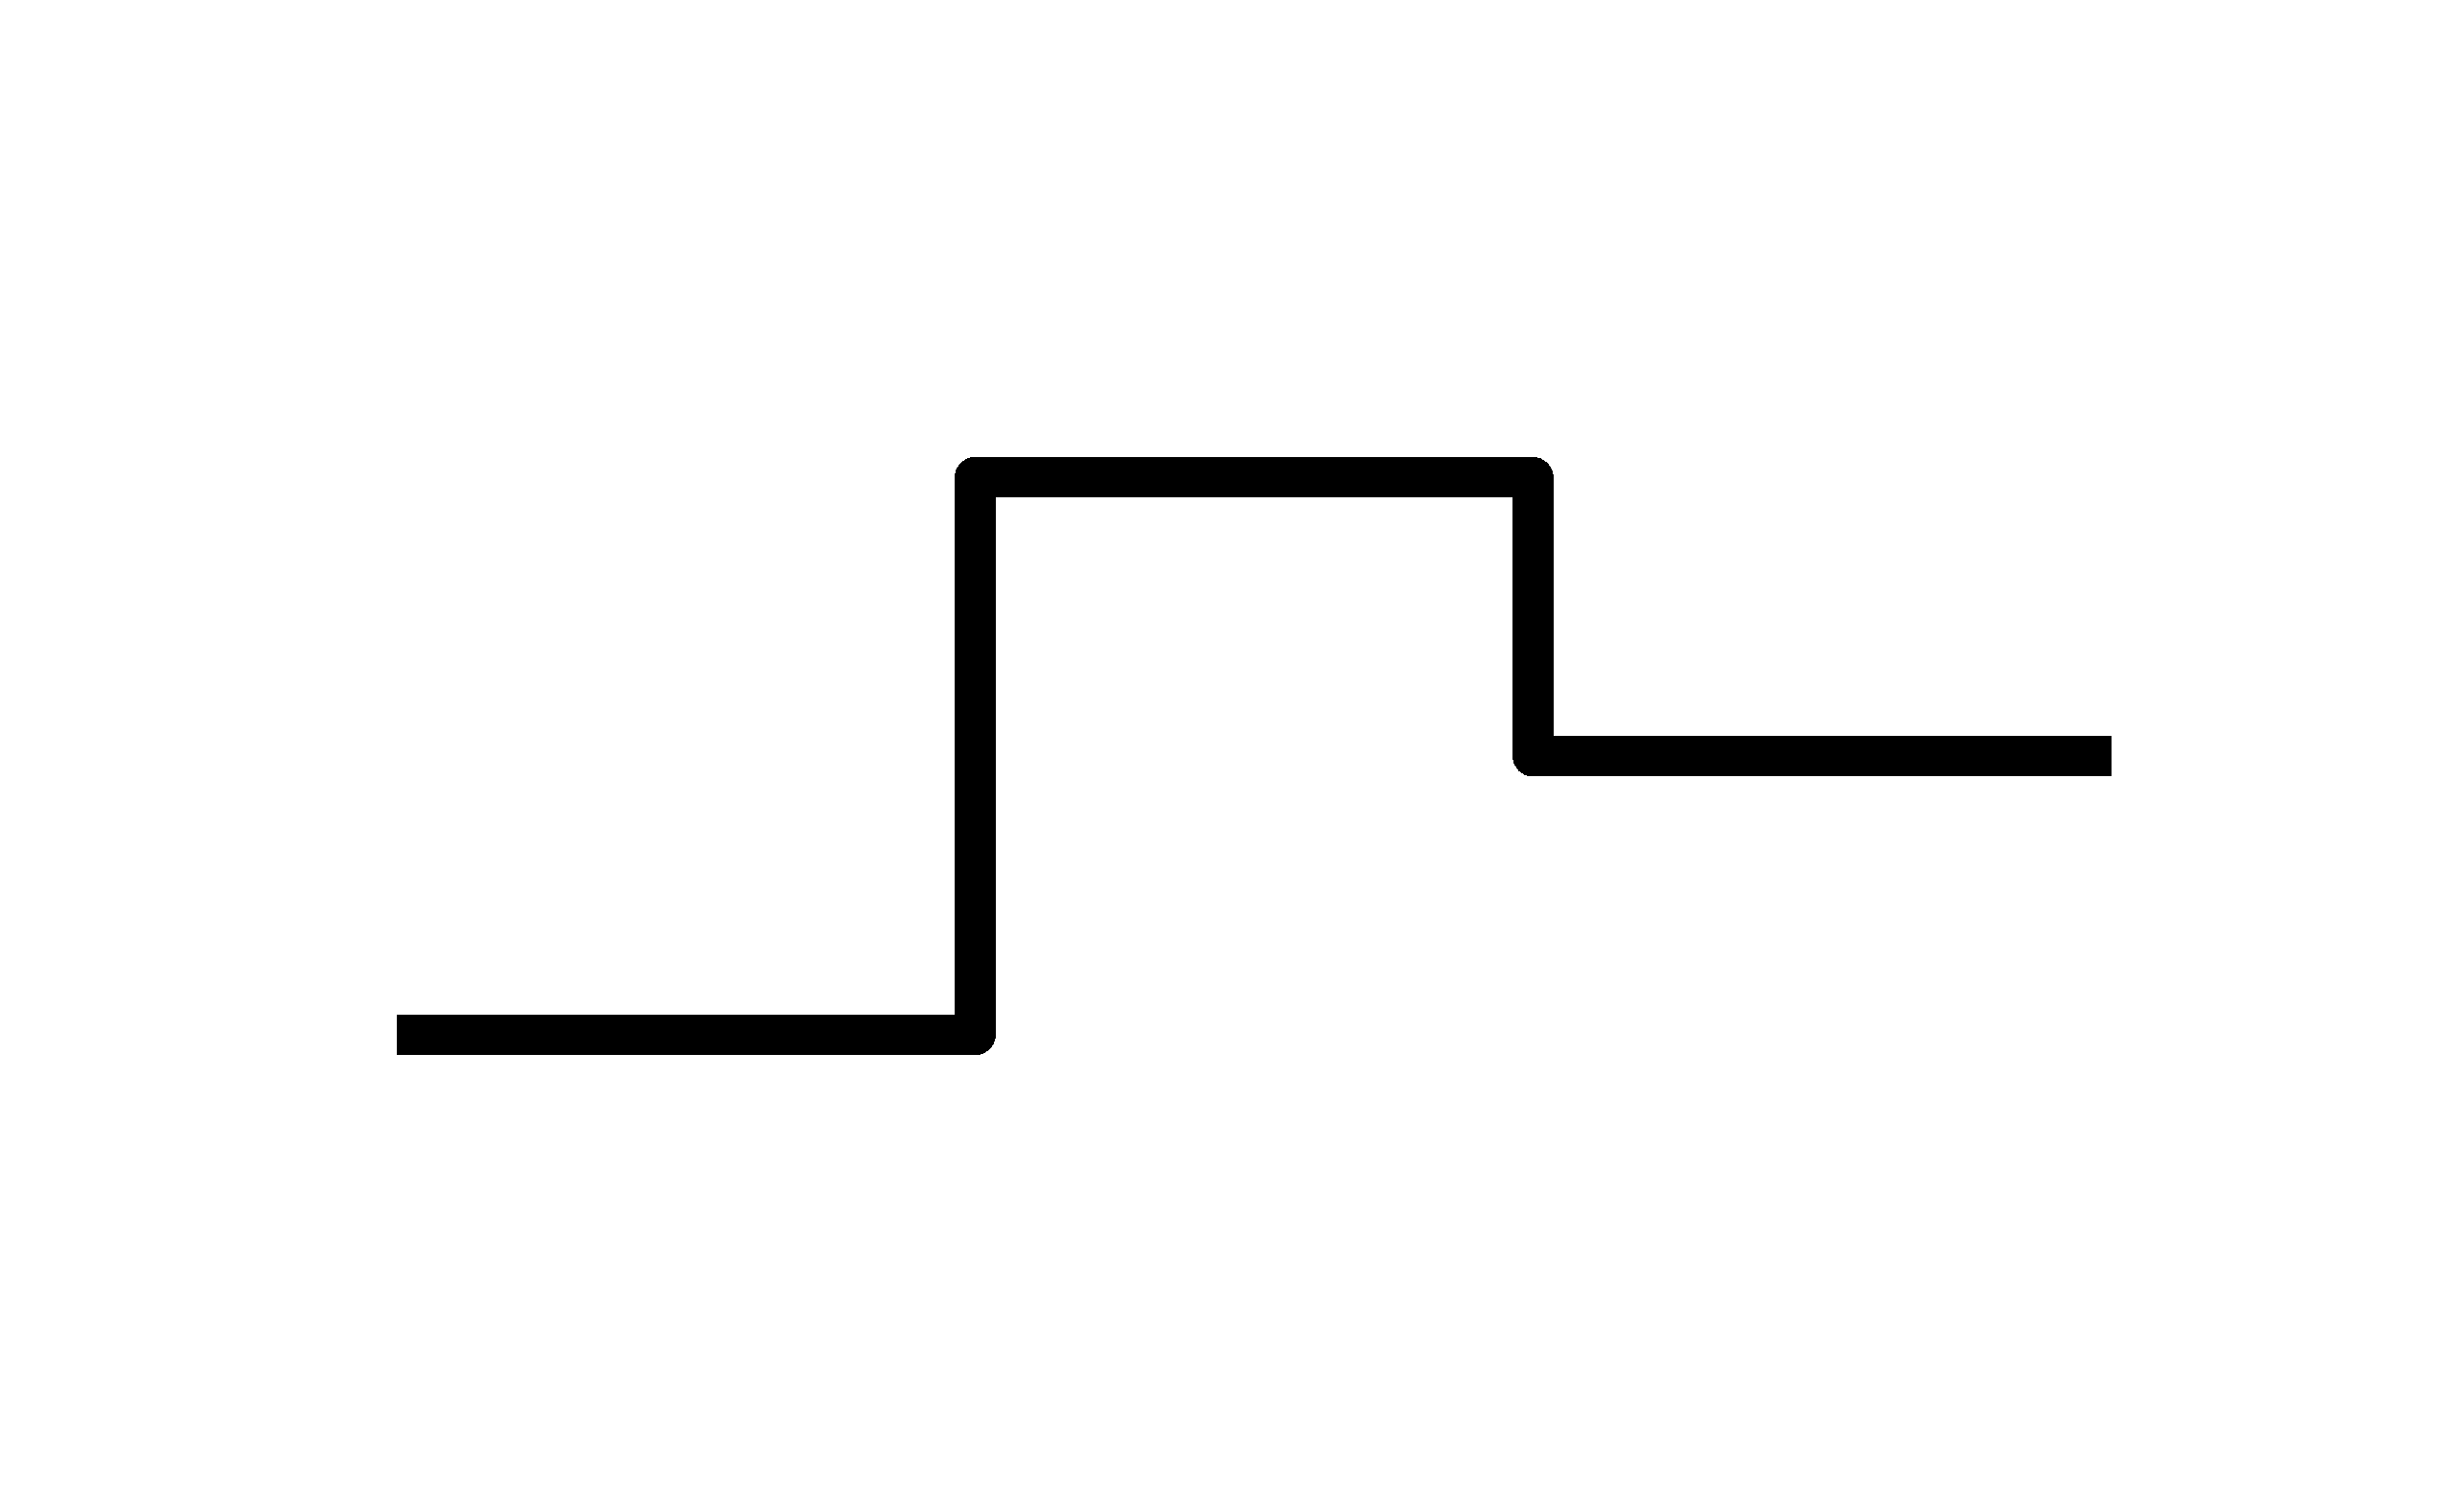
\includegraphics[width=.252\linewidth]{supplement/beta_cluster_example_2/pictures/17/state_cluster_shapes_3.pdf} &
    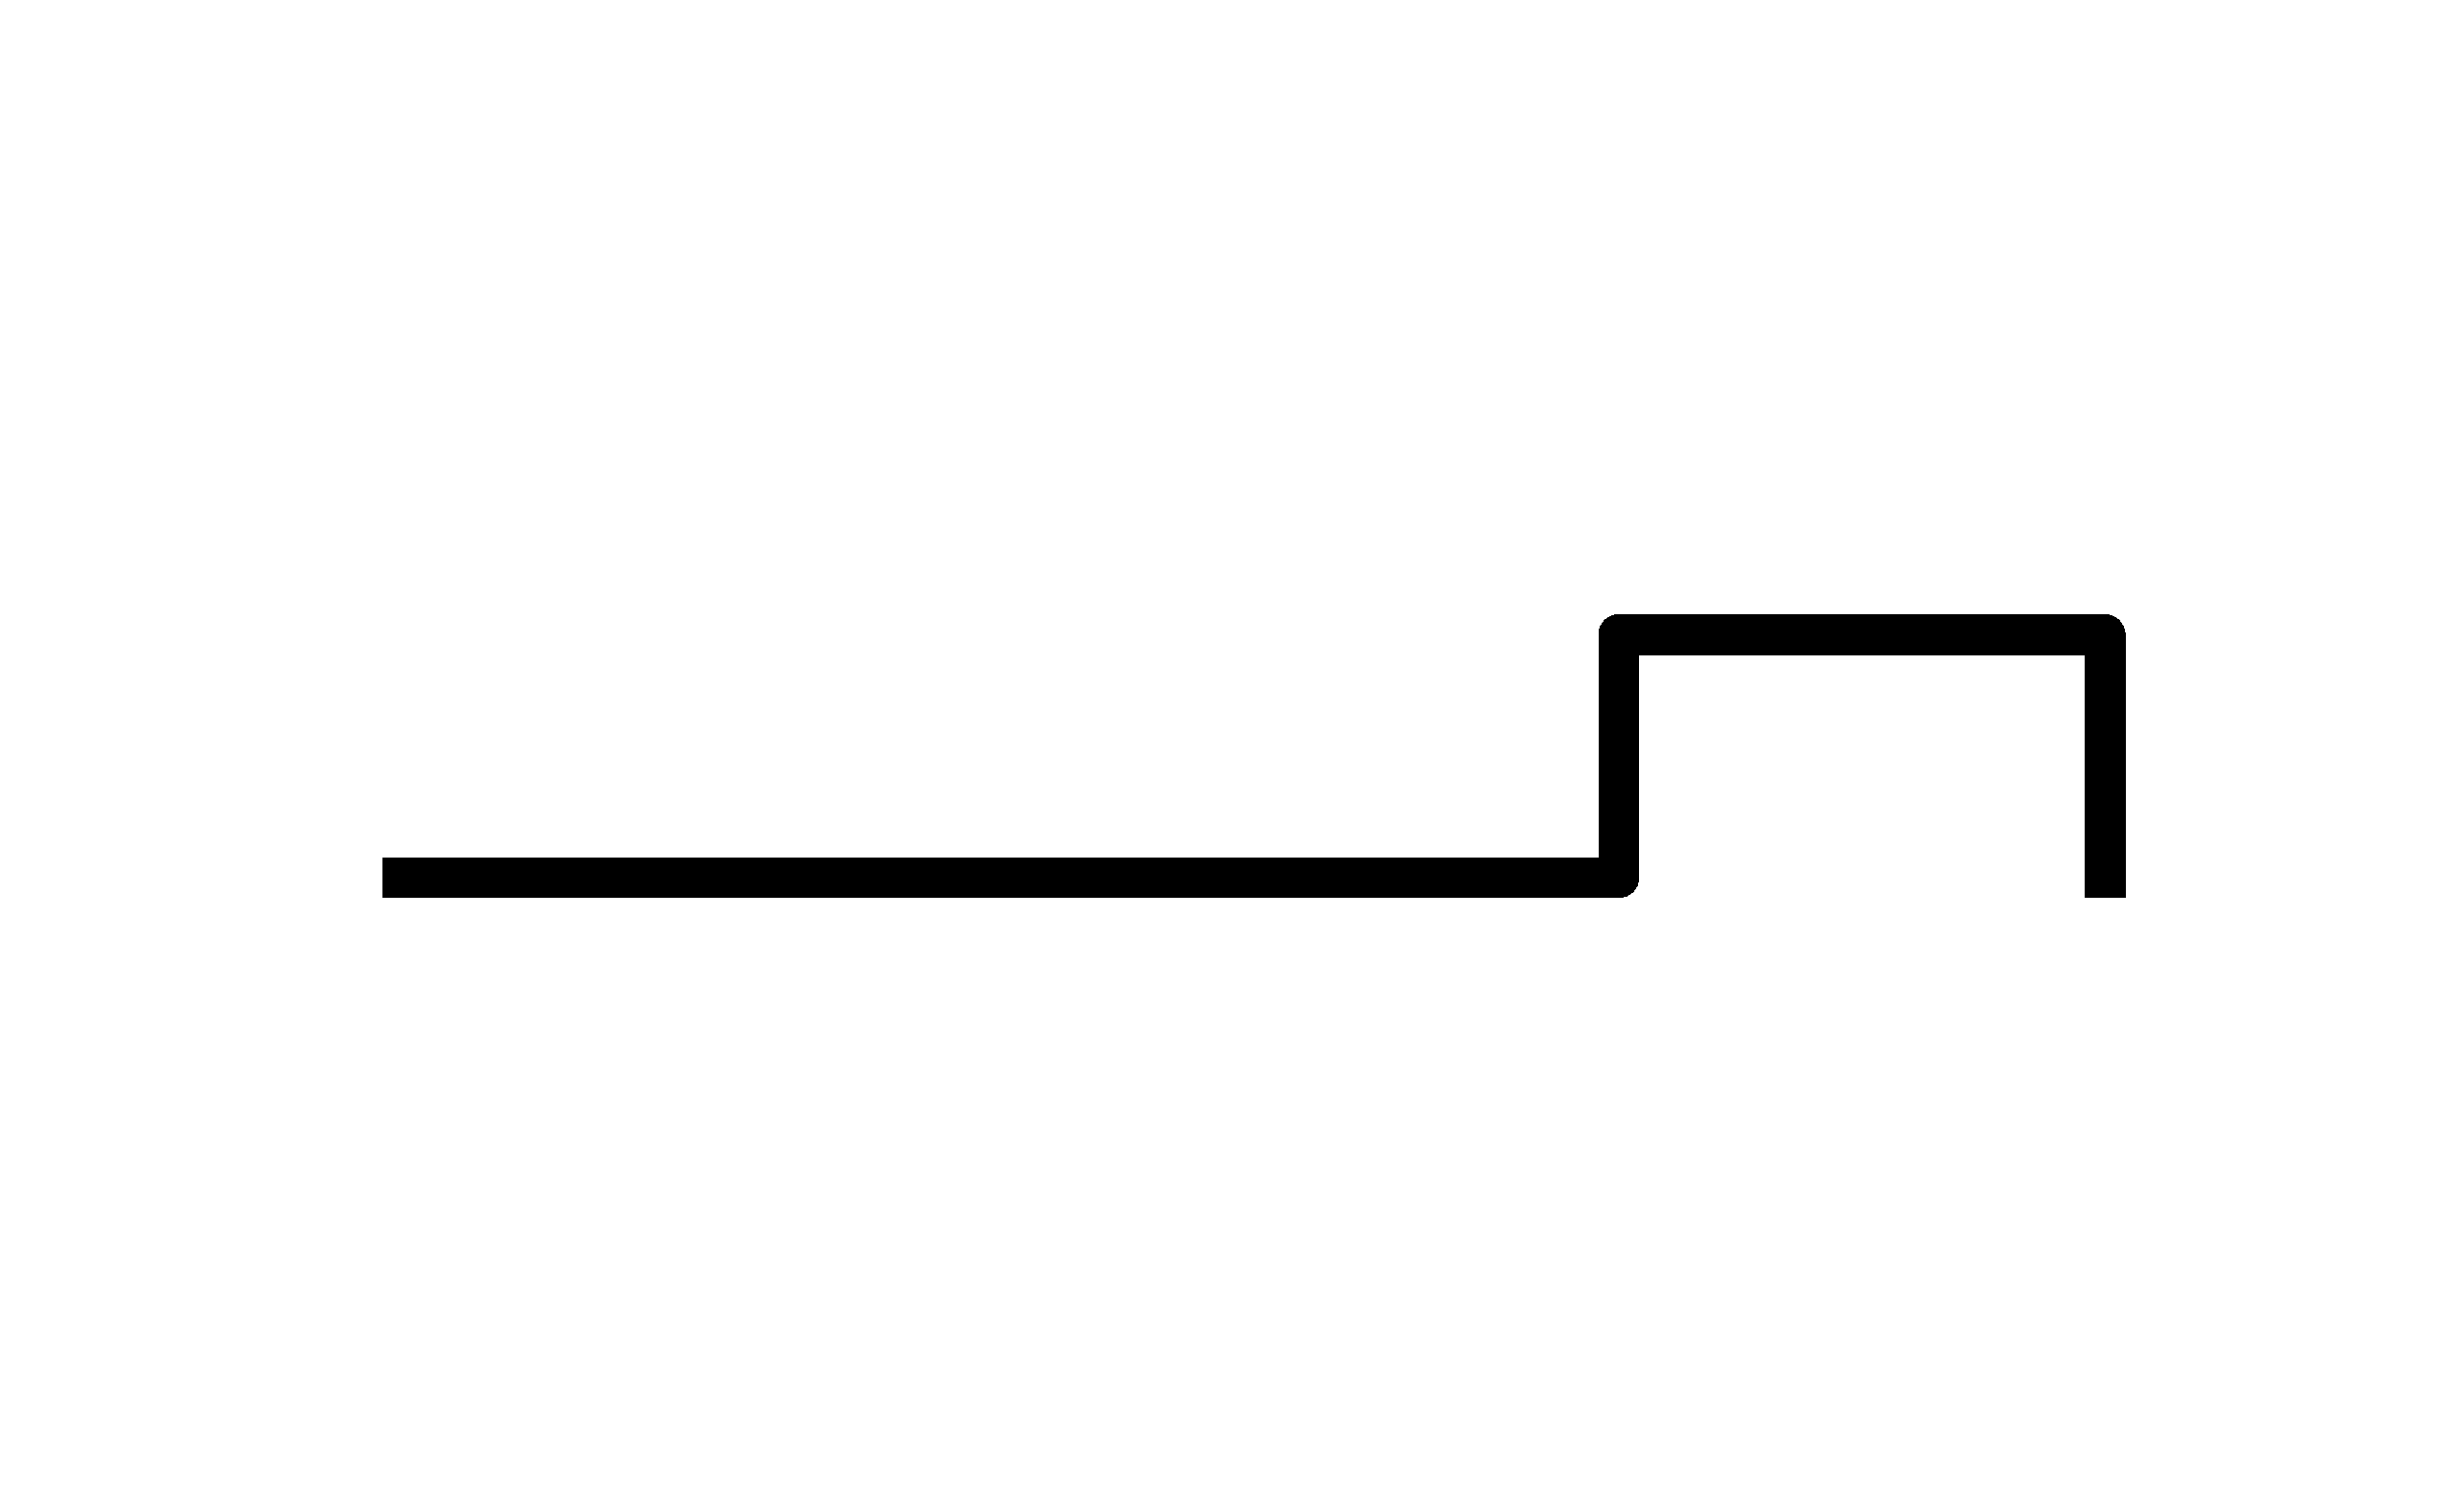
\includegraphics[width=.252\linewidth]{supplement/beta_cluster_example_2/pictures/17/state_cluster_shapes_4.pdf} &
    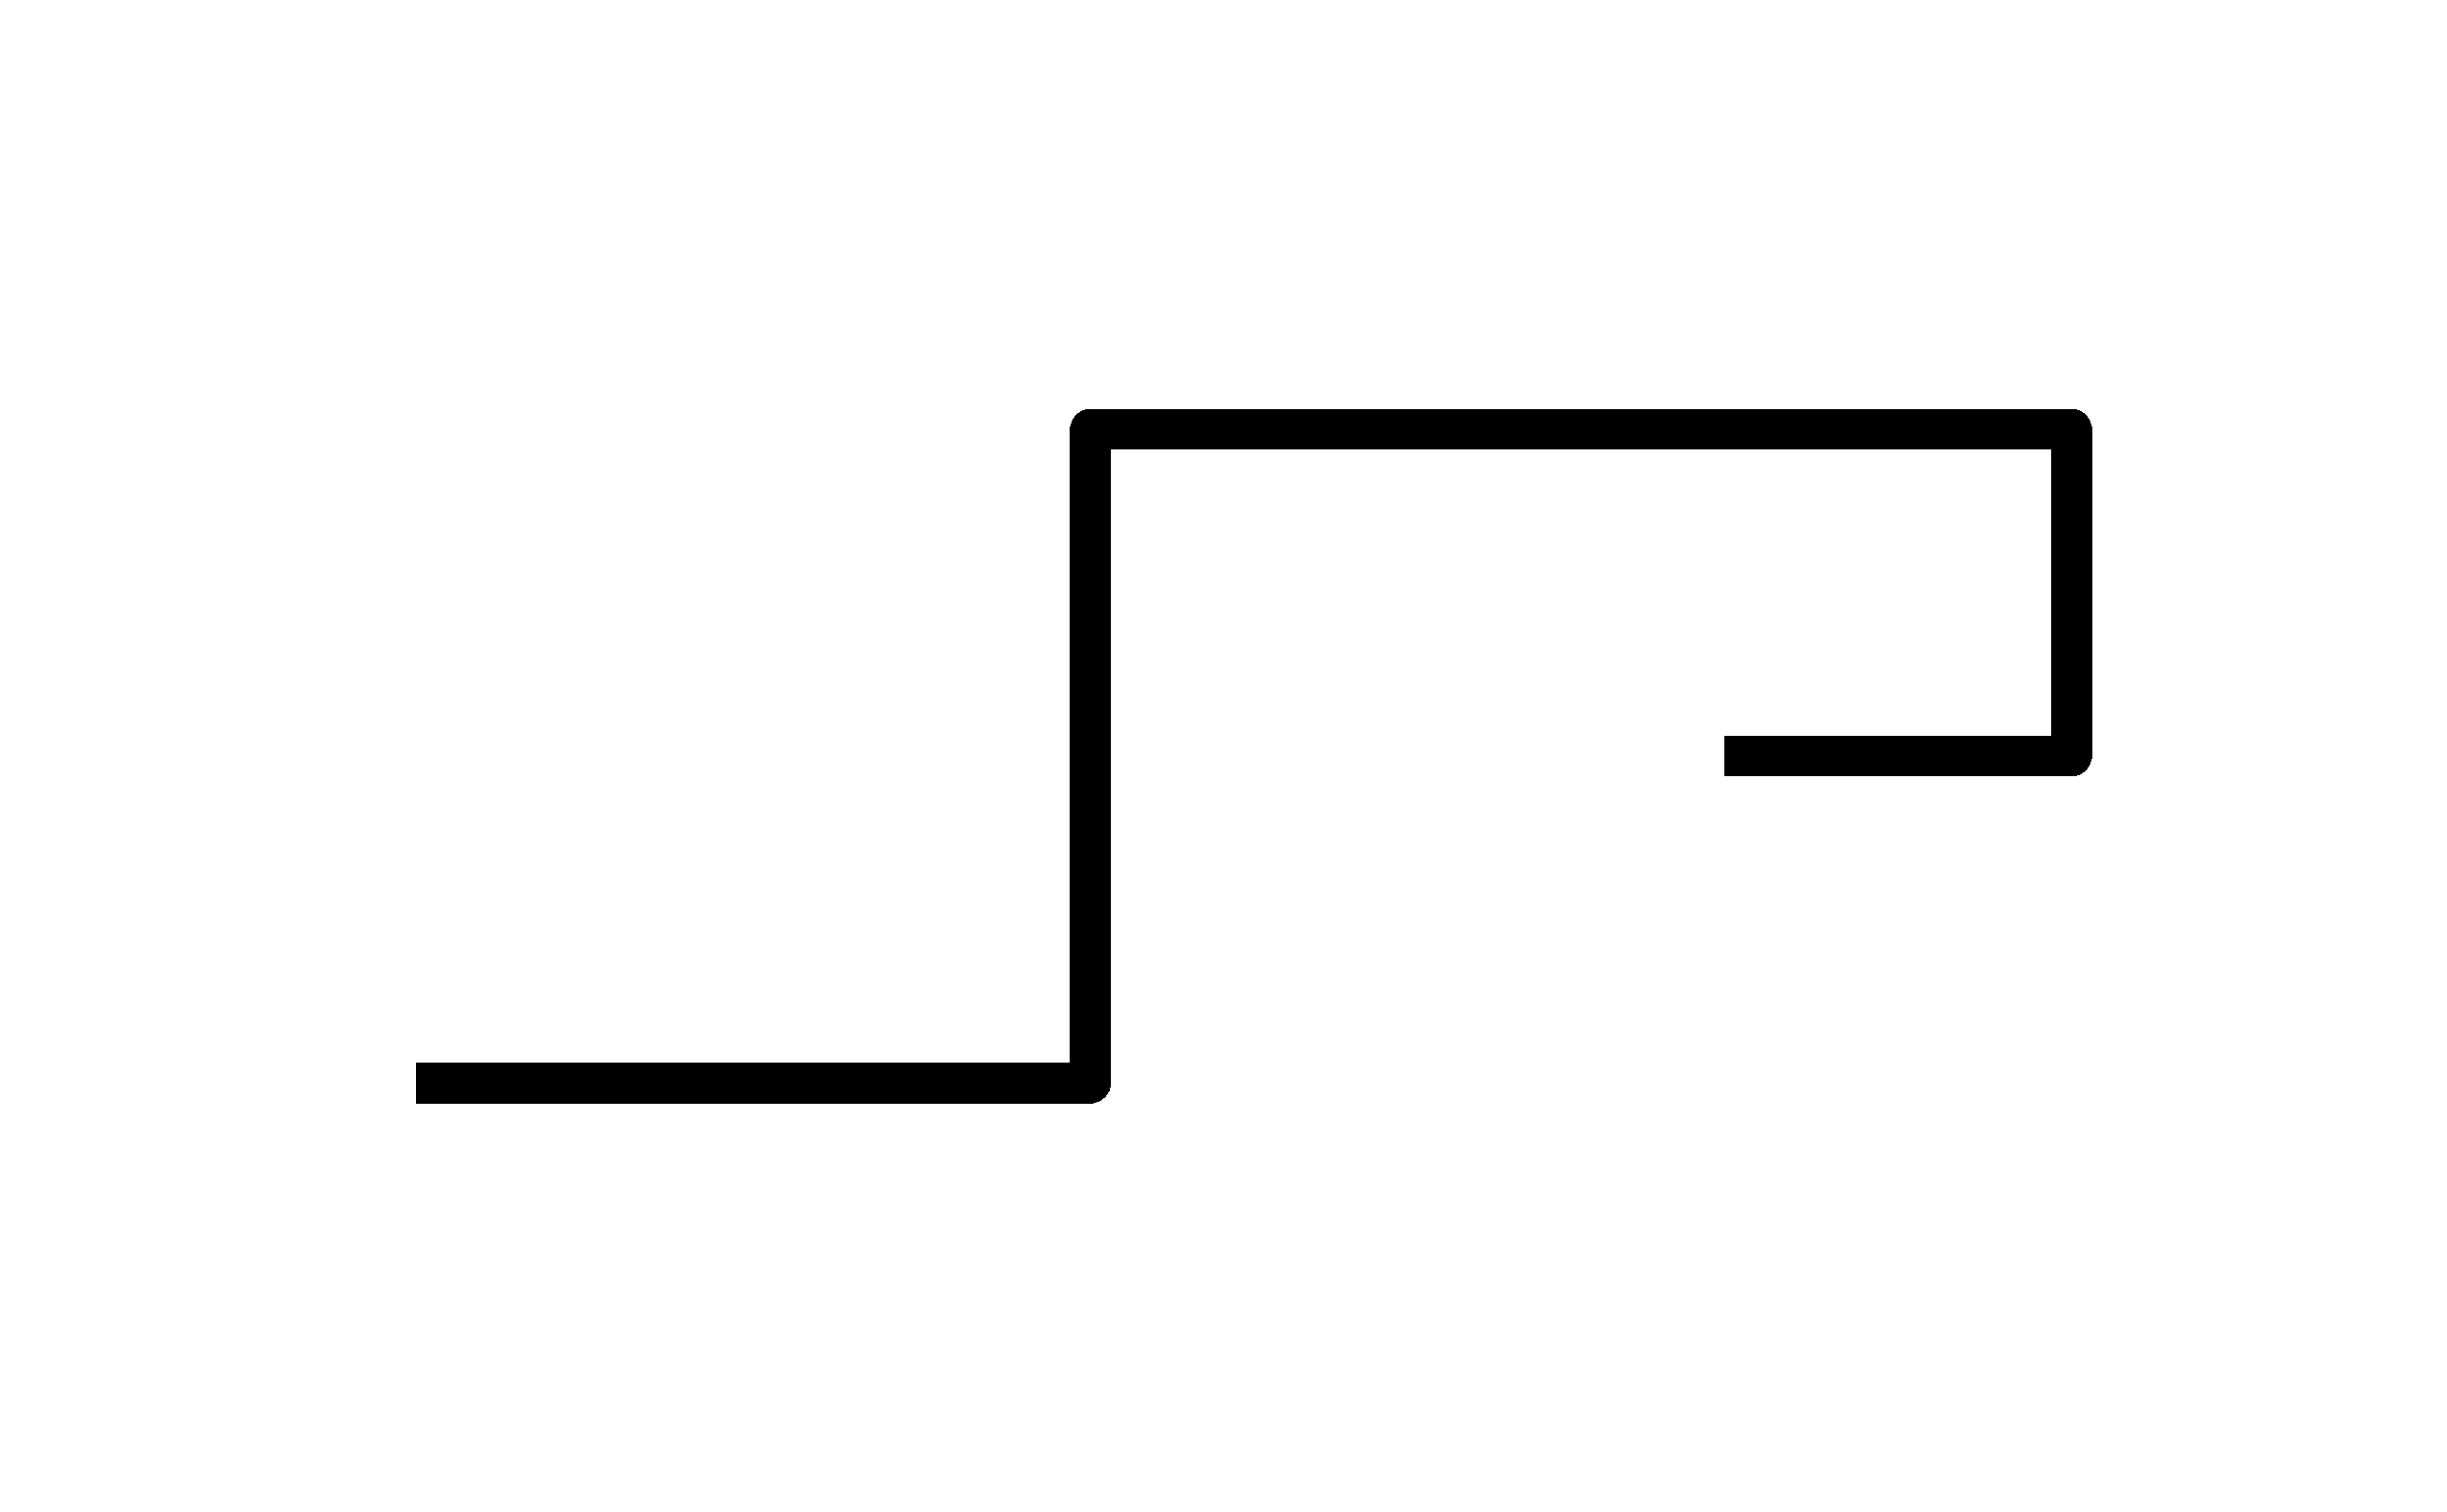
\includegraphics[width=.252\linewidth]{supplement/beta_cluster_example_2/pictures/17/state_cluster_shapes_5.pdf} 
  \end{tabular}
}
%
\inlineframebox{\B{Intermediate Cluster} $c_{18}$} {
  \begin{tabular}{ c c c }
    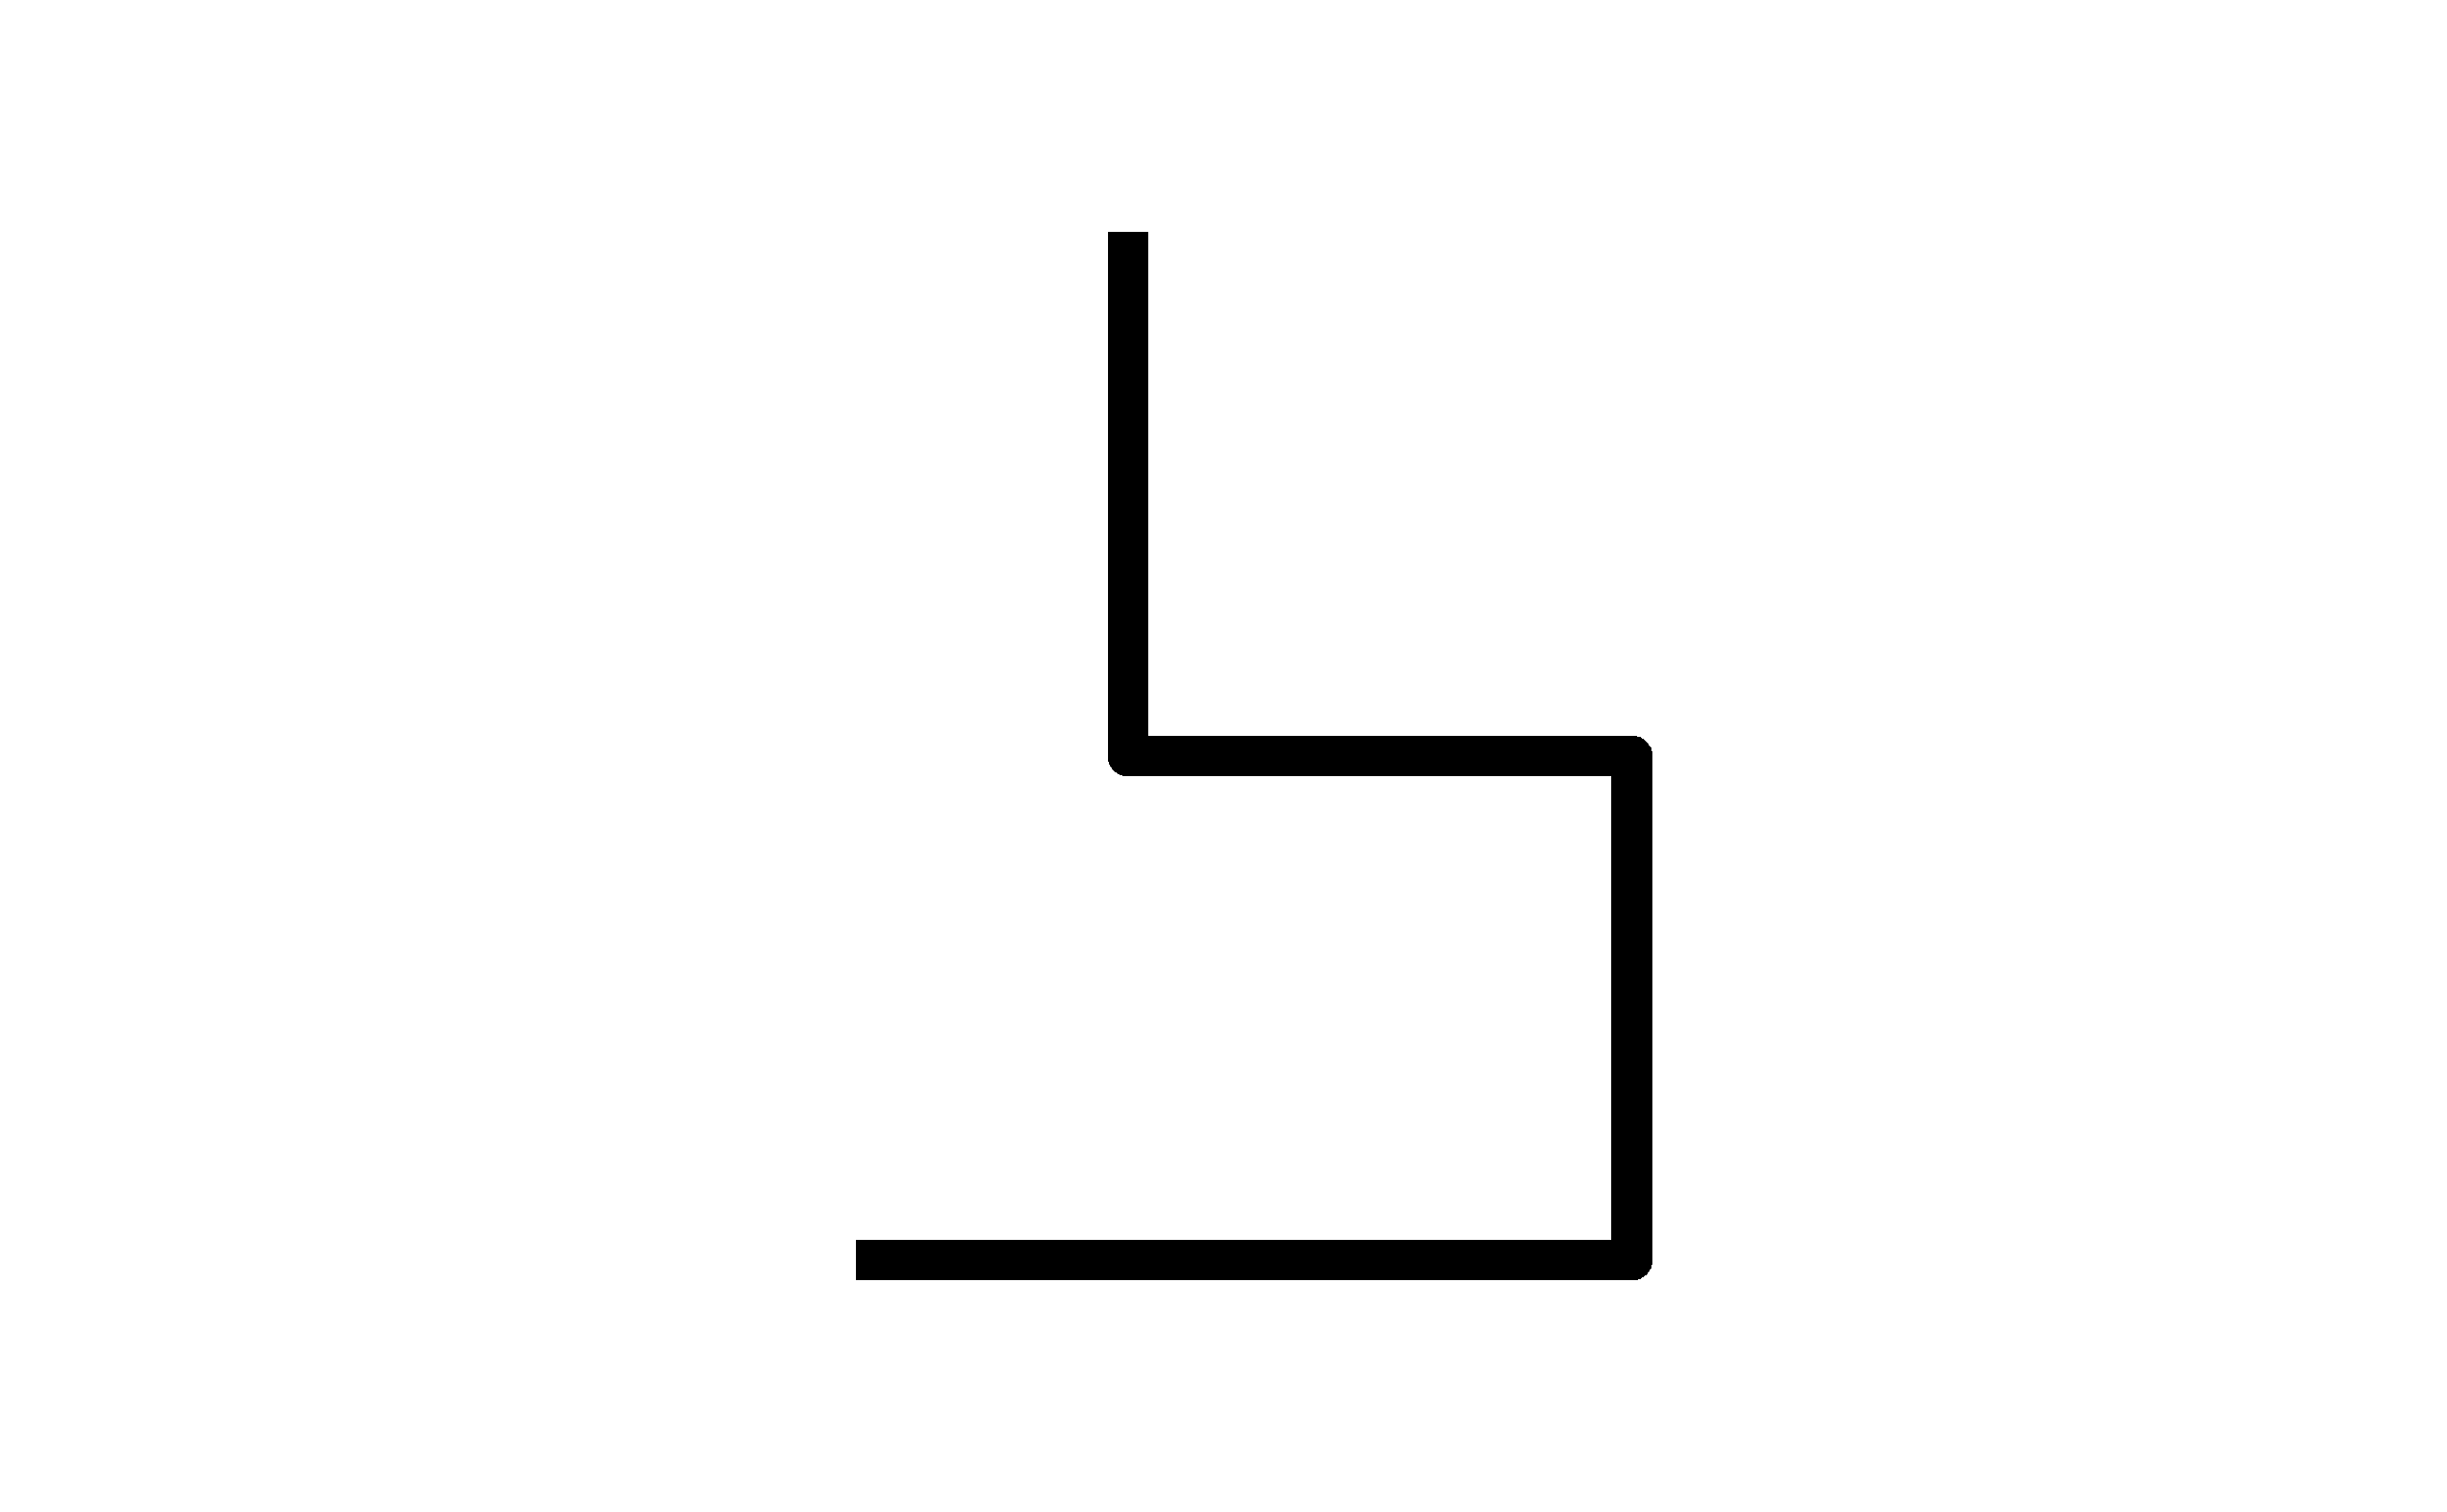
\includegraphics[width=.252\linewidth]{supplement/beta_cluster_example_2/pictures/18/state_cluster_shapes_0.pdf} &
    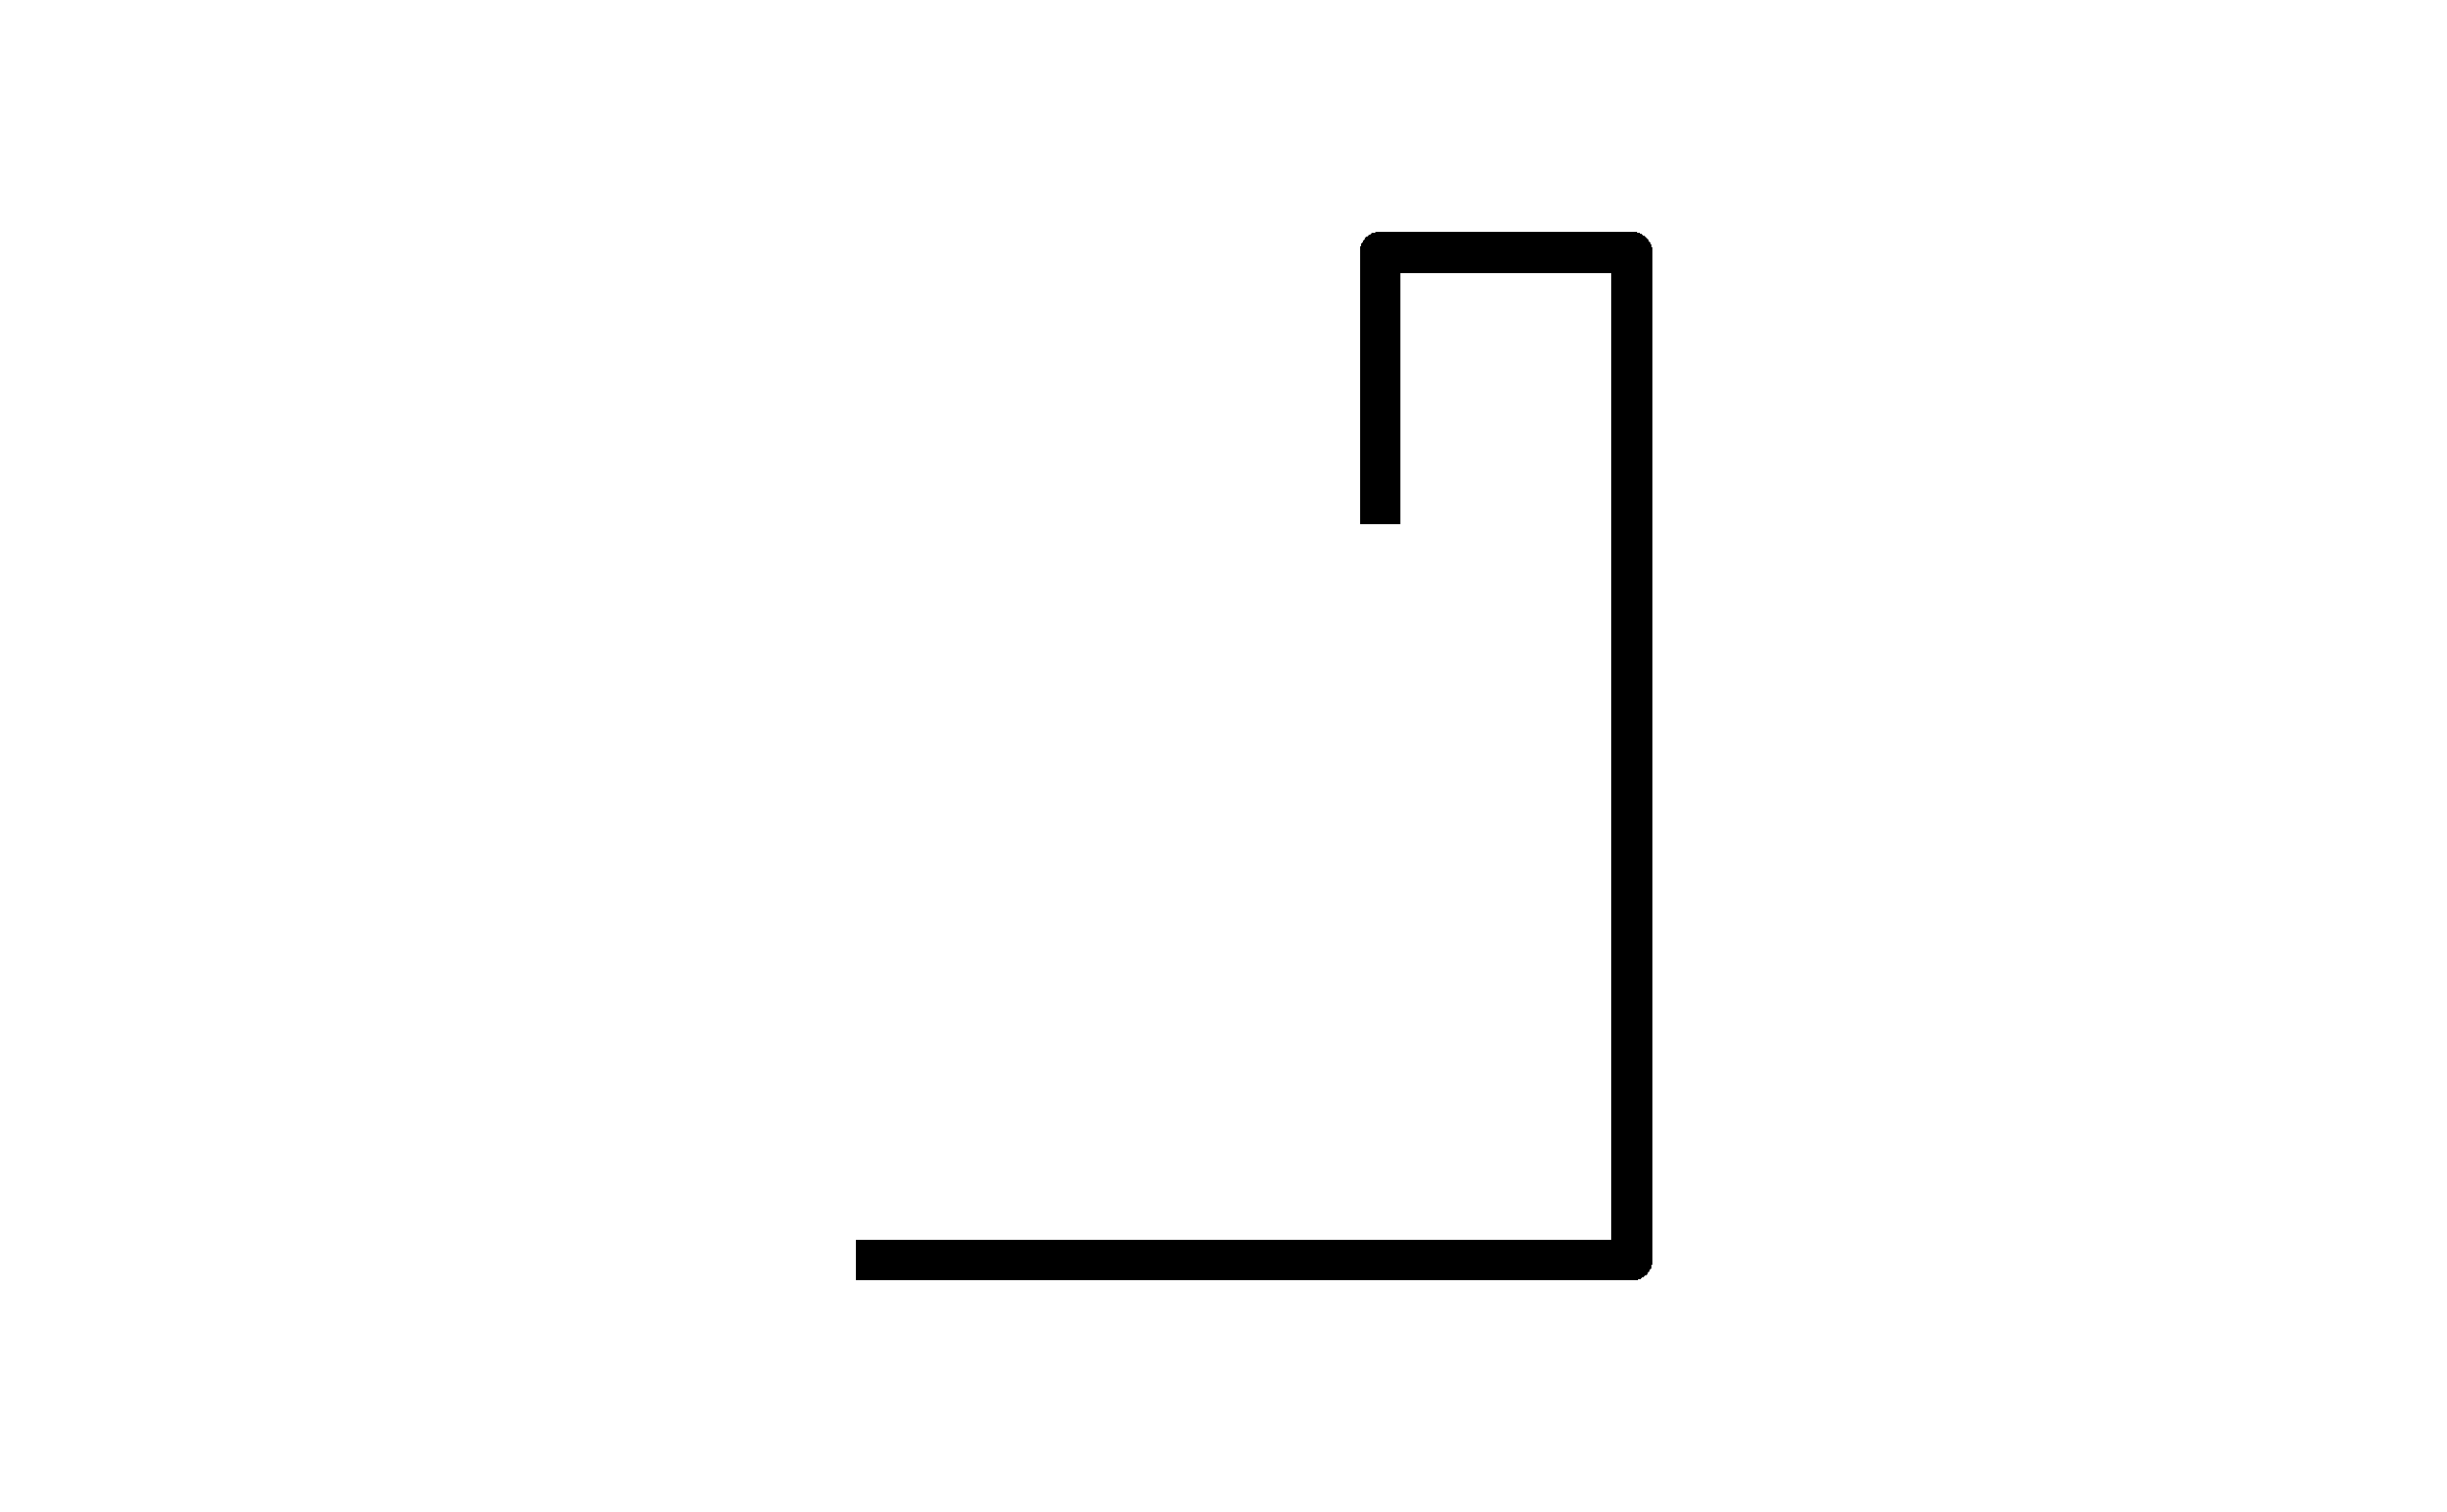
\includegraphics[width=.252\linewidth]{supplement/beta_cluster_example_2/pictures/18/state_cluster_shapes_1.pdf} & 
    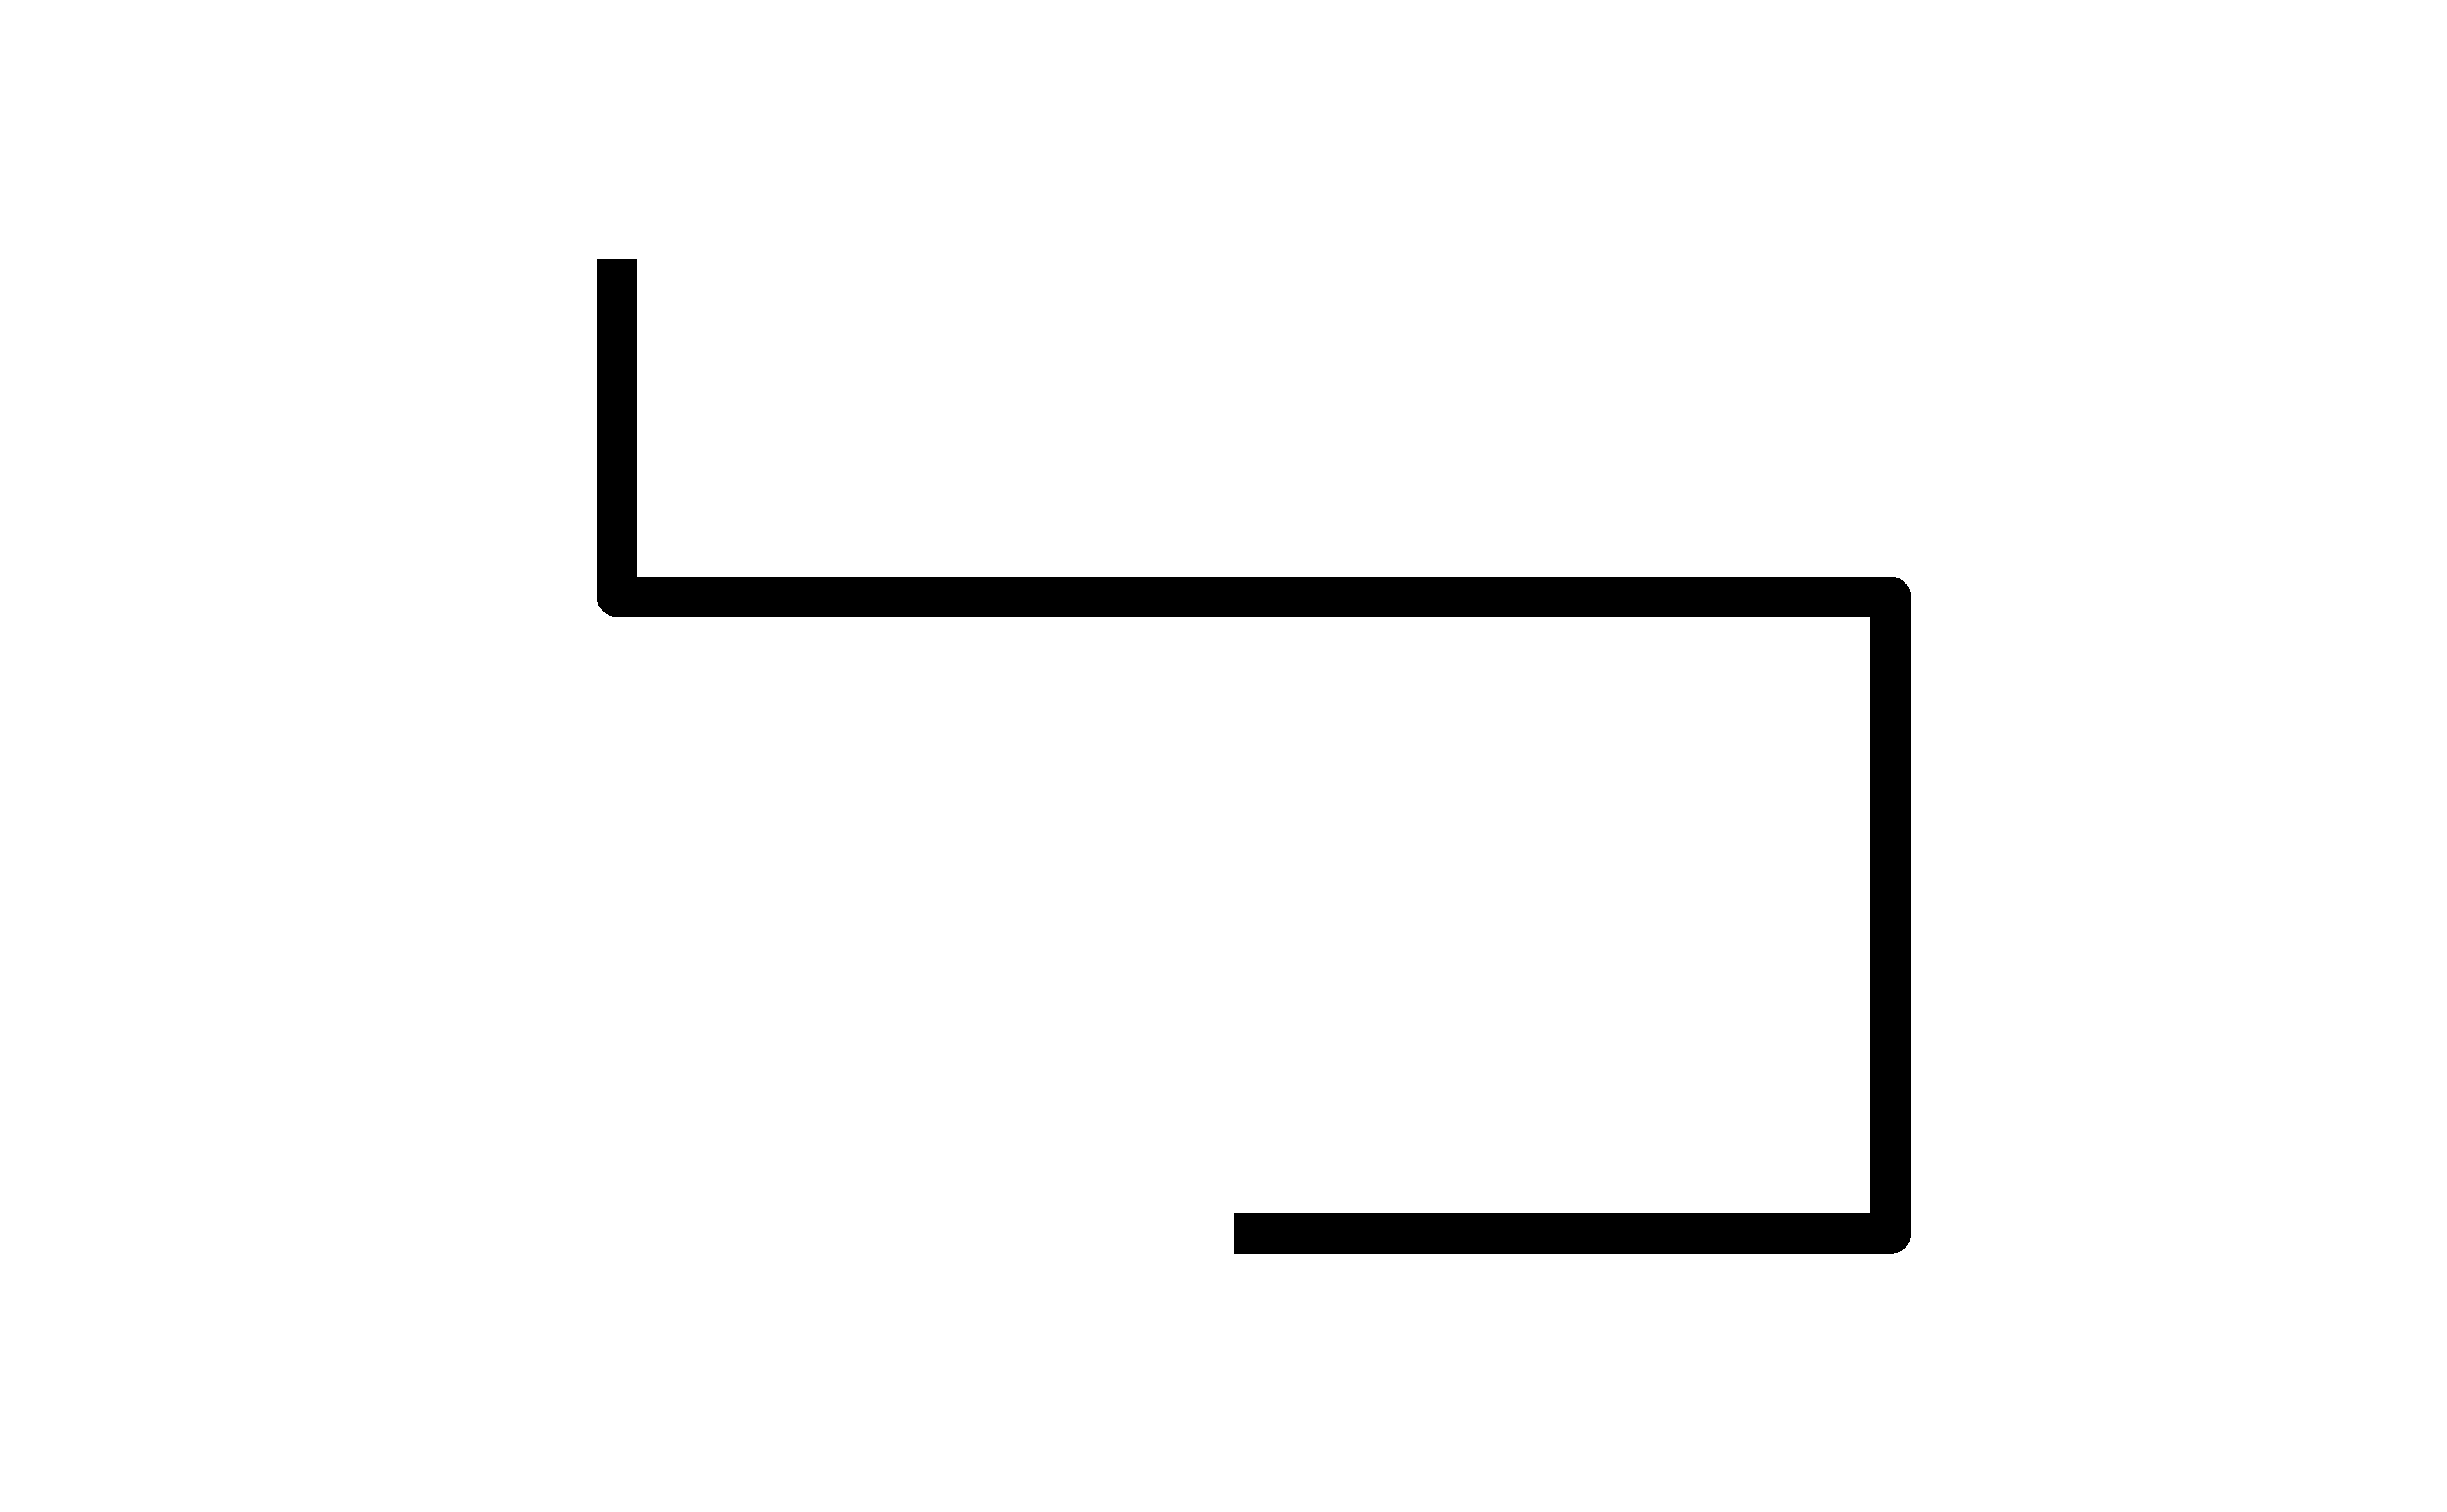
\includegraphics[width=.252\linewidth]{supplement/beta_cluster_example_2/pictures/18/state_cluster_shapes_2.pdf} \\
    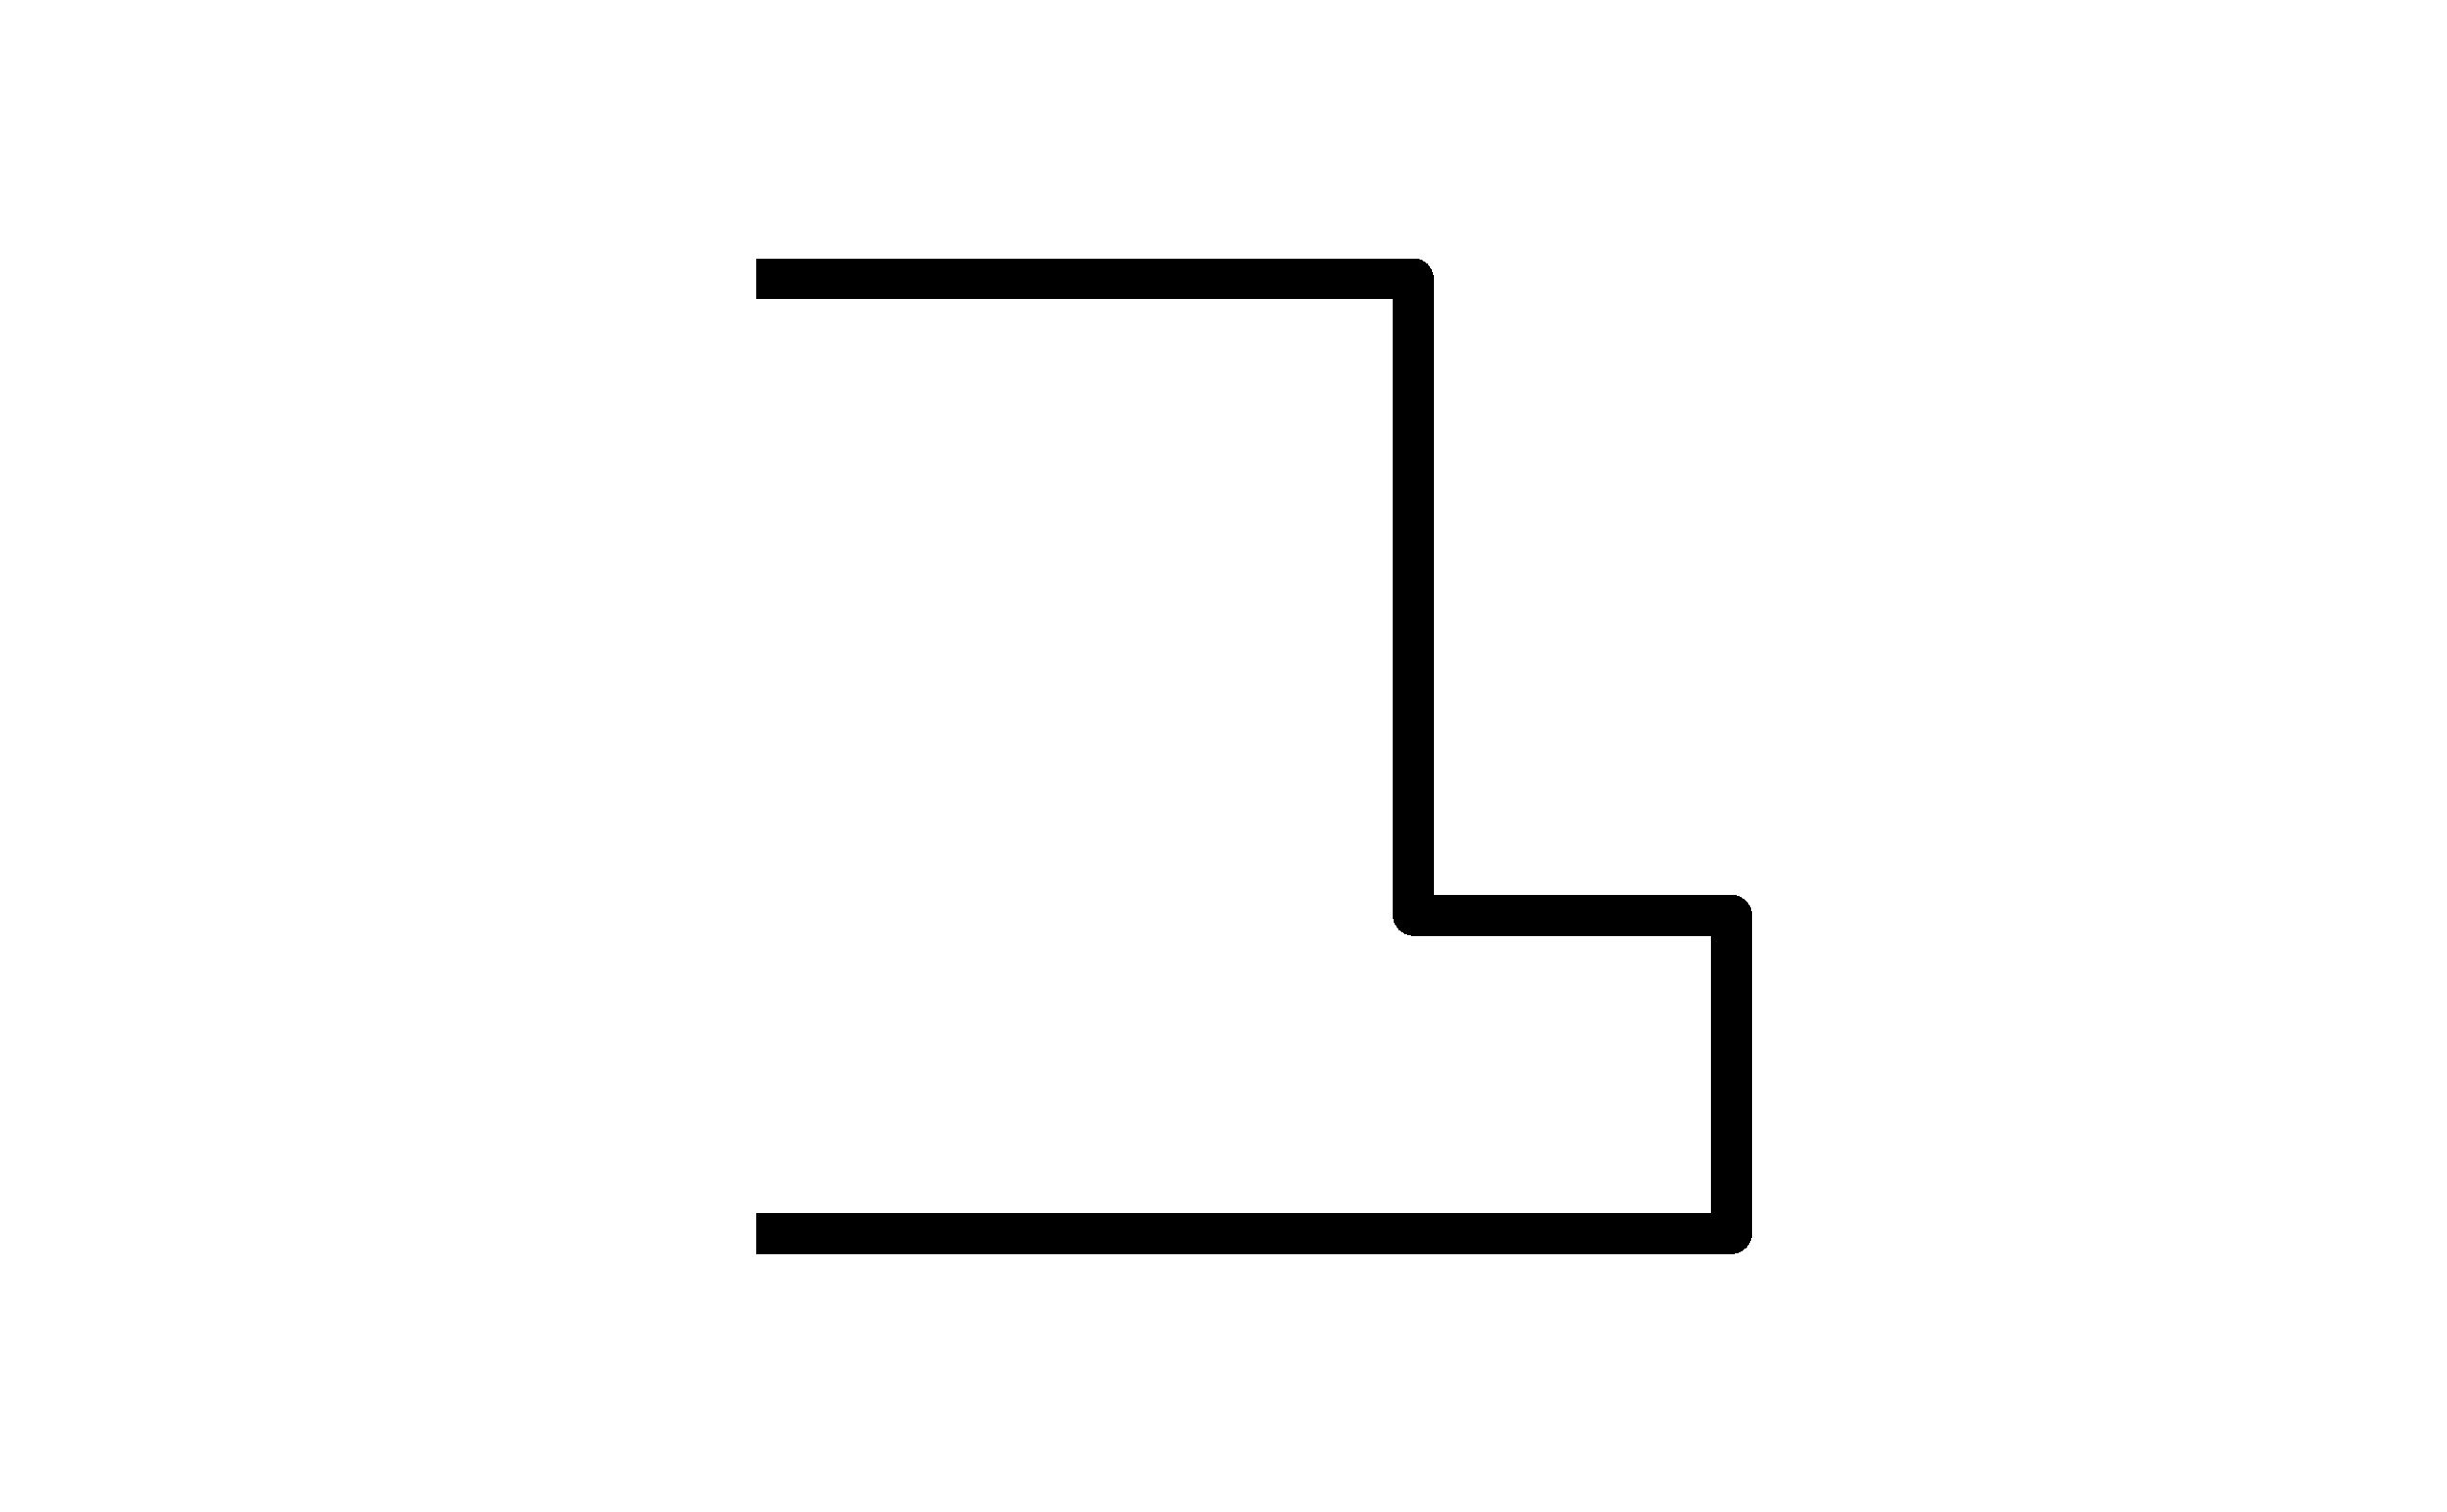
\includegraphics[width=.252\linewidth]{supplement/beta_cluster_example_2/pictures/18/state_cluster_shapes_3.pdf} &
    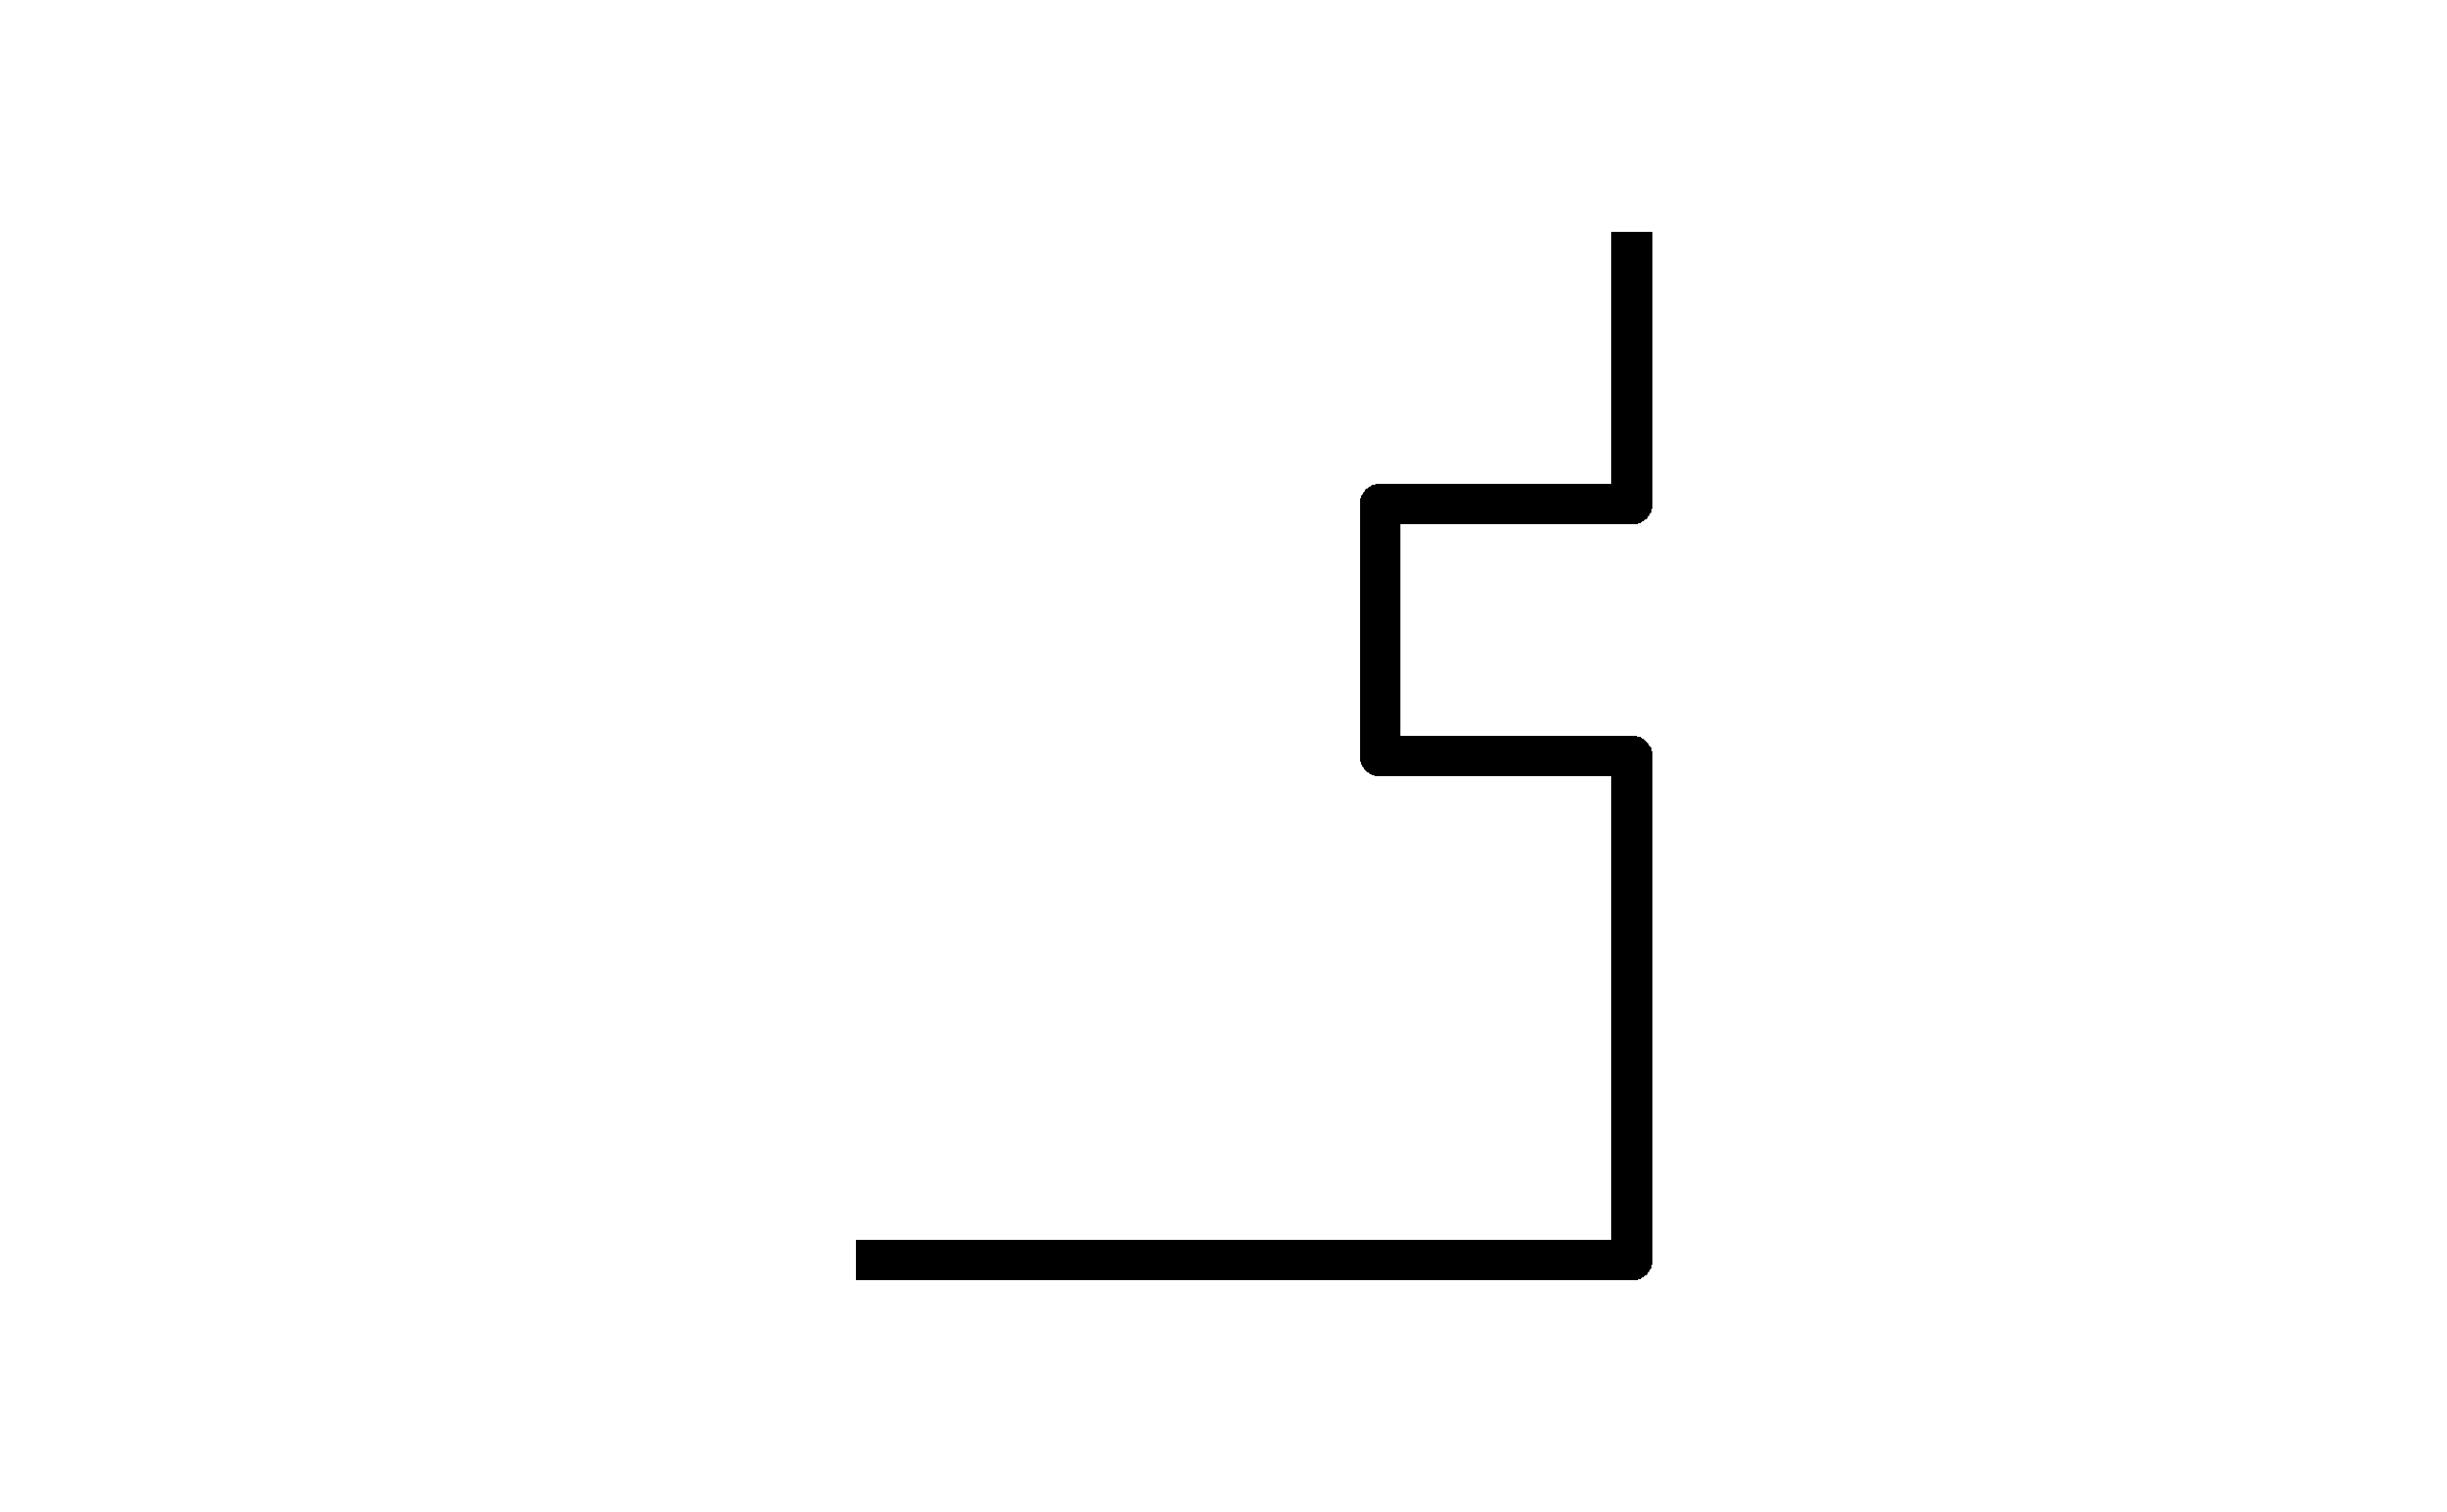
\includegraphics[width=.252\linewidth]{supplement/beta_cluster_example_2/pictures/18/state_cluster_shapes_4.pdf} &
    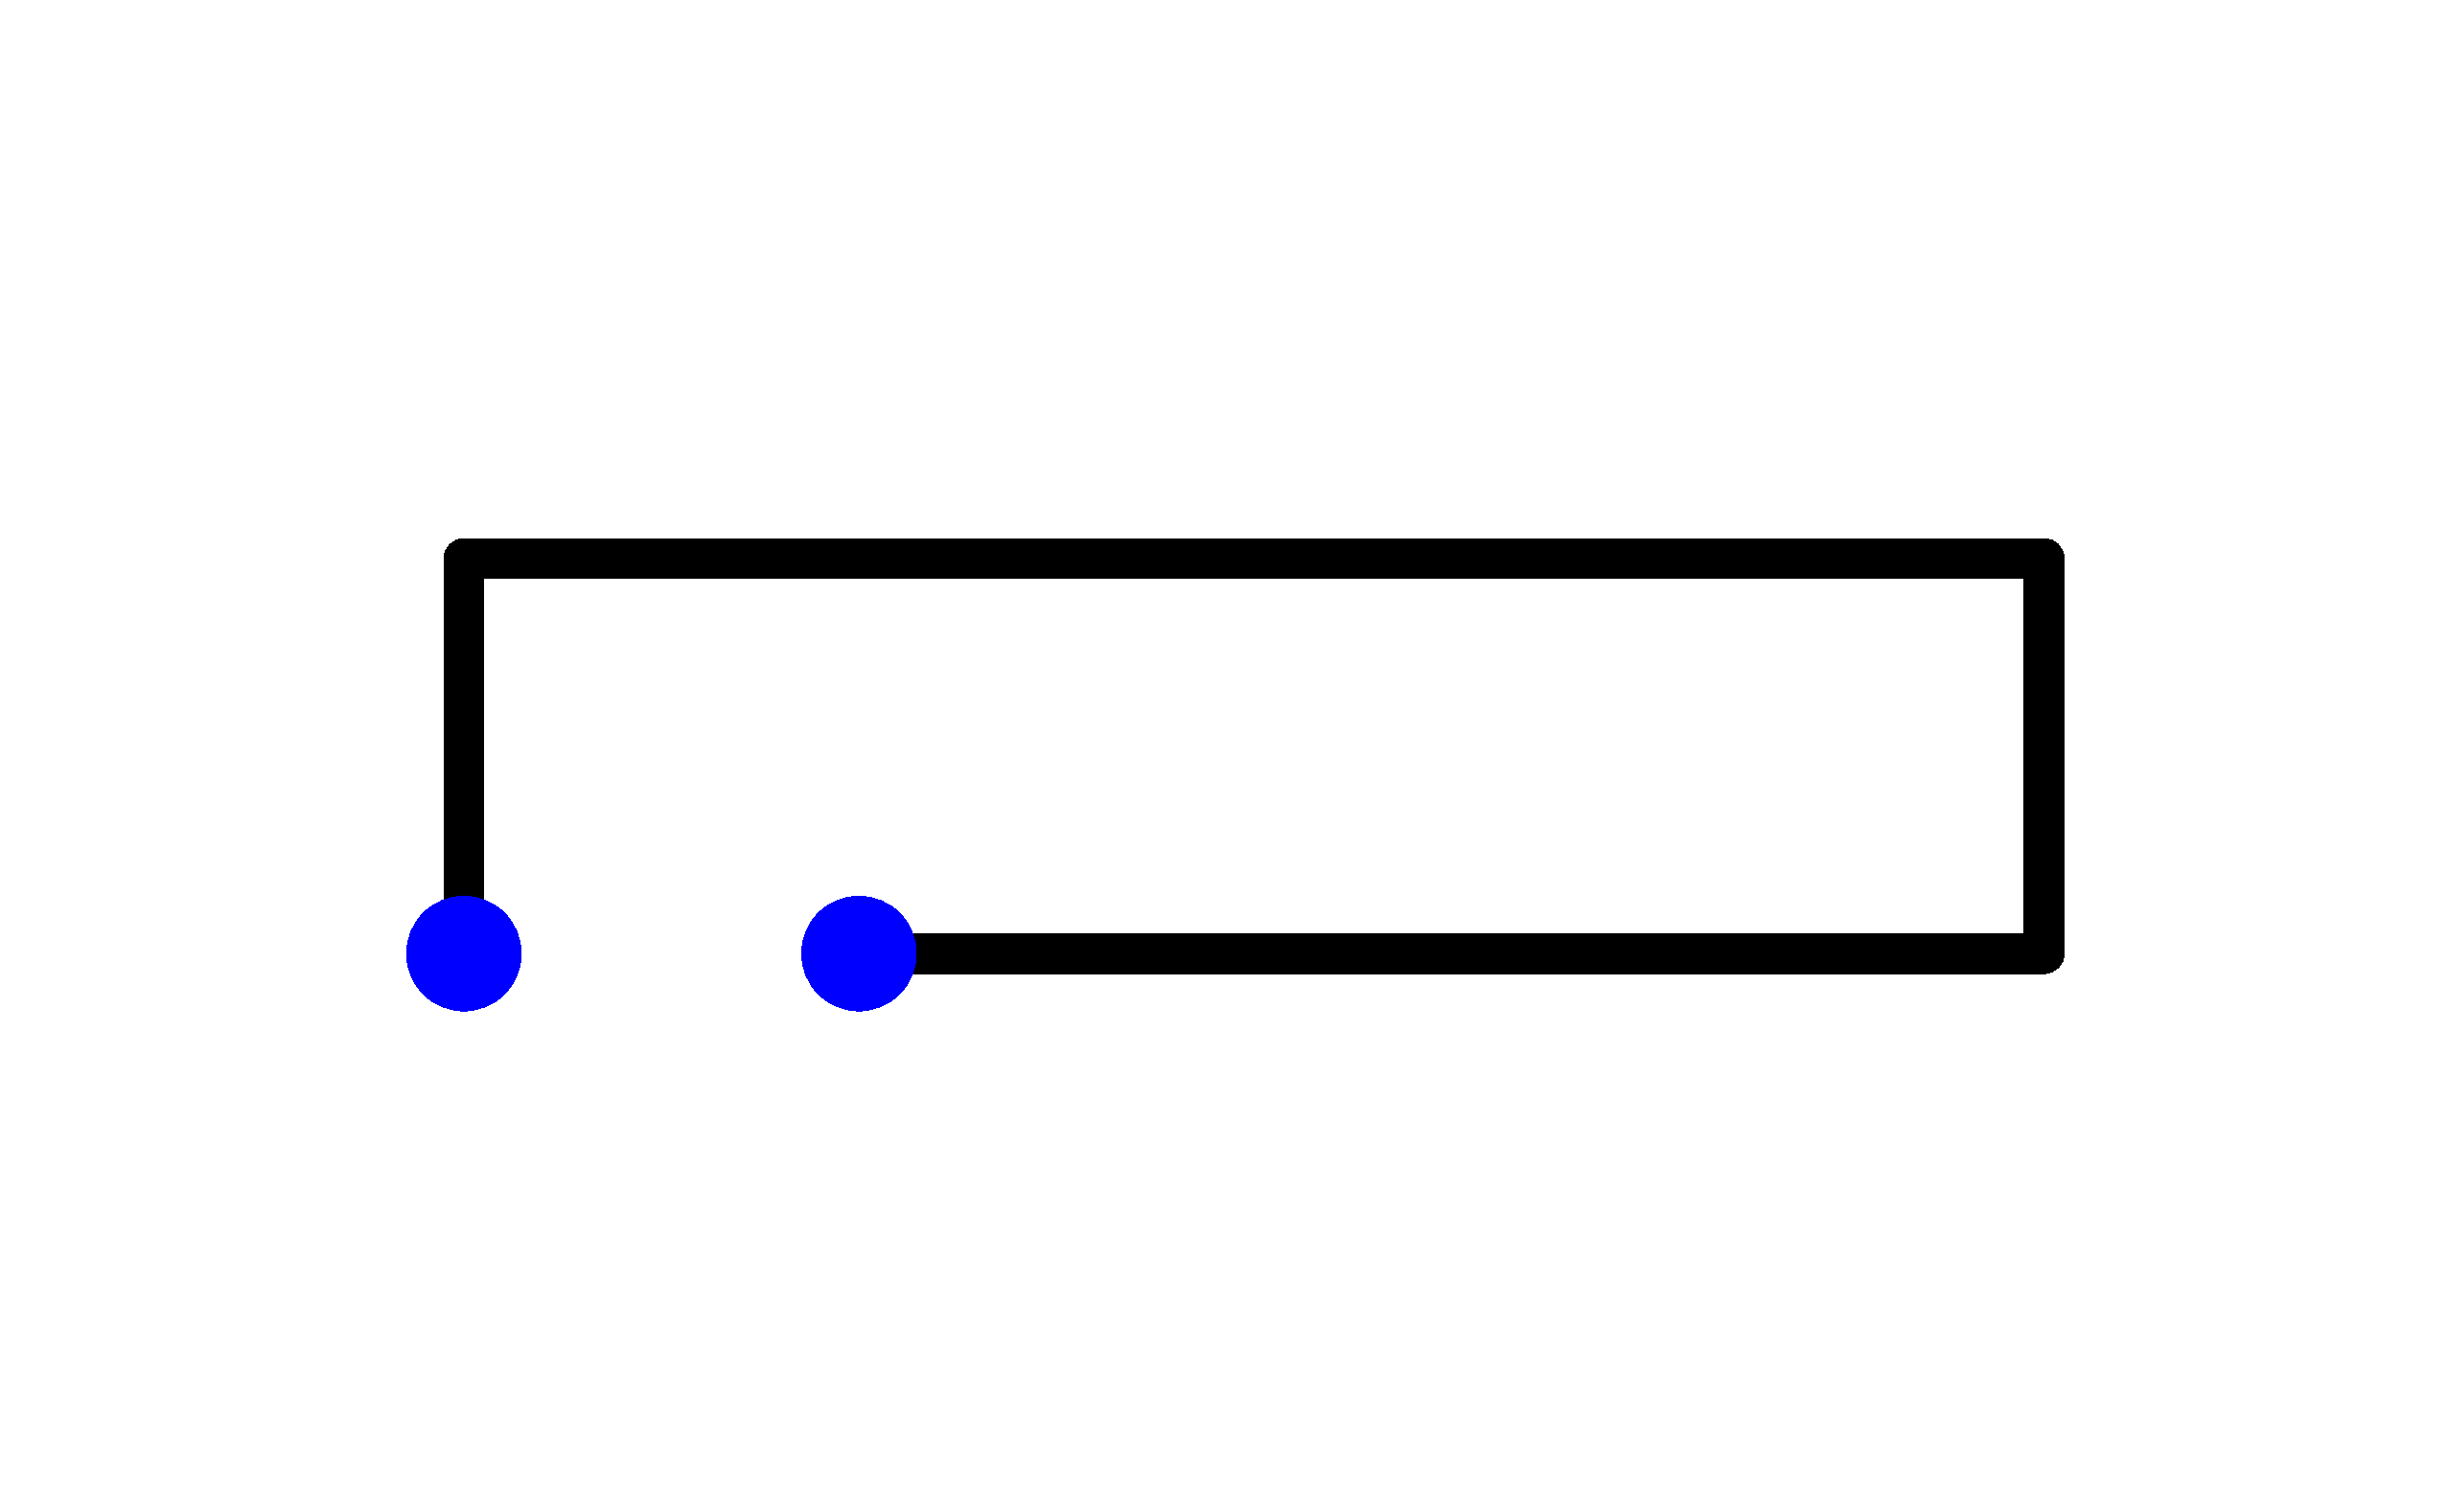
\includegraphics[width=.252\linewidth]{supplement/beta_cluster_example_2/pictures/18/state_cluster_shapes_5.pdf} 
  \end{tabular}
}
%
Clearly the folding pathway is dominated by the formation of the turn. This implies that the formation of the turn in the $\beta$-hairpin is a nucleation event, a necessary first step for the folding process. 

The folding kinetics can be computed using the quasi-steady-steady approximation. Grouping the intermediate states as $c_\chem{I} = \braces{c_{17}, c_{18}}$, the final state $c_\chem{F} = \braces{c_{11}}$ and all other clusters as random coil states $c_\chem{R}$ we have
%
\inlinembox{Macrostate model for $\beta$-hairpin}{\TIKZbetahairpinMacrostates}
%
The forward and backwards transitions were calculated to be
\begin{equation}
  \B{S} =
  \begin{bmatrix}
    0.54042 & 0.39912 & 0.06046 \\
    0.00713 & 0.99266 & 0.00021 \\
    0.00005 & 0.00001 & 0.99995 \\
  \end{bmatrix}
\end{equation}
with the rows ordered as $\brackets{ c_\chem{R}, c_\chem{I}, c_\chem{F} }$.

We stress that these predicted transitions are a coarse-graining of the real kinetics since we have assumed the states equilibrate before transitioning into a different macrostate. Nevertheless, the approximation is validated by the observation that at the observed temperature, the slowest eigenmodes dominate the kinetics. 

\section {Remarks}

When the number of microstates is large, the eigendecomposition could take an inordinate amount of computation. Thankfully, once $\phi$ is chosen, only the largest eigenpairs need to be found. In general, the full eigendecomposition is unnecessary. There exist techniques like the Lanczos routine that extract only the larger eigenpairs.\cite{komzsik_lanczos_1987} These techniques work well with the matrices used in the MSC algorithm; the Lanczos algorithm works with non-Hermitian matrices and excels when the matrices are sparse and the eigenvalues are not degenerate.

It is worth noting that the macrostates obtained did not use the equations of motion, only the time-series data. This gives the technique  wide applicability, extending beyond the domain of biophysical simulations. While the systems studied here were small, the MSC method should scale well to larger more complicated sets of conformational microstates. The limit of the application appears to be the ability of the researcher to extract meaningful data out of the clusters once they have been found. For example, in a larger off-lattice model of protein folding, the full state space of each of the $3N$ residues' coordinates may be unnecessary. In this case, a relative set of microstates may be more useful, say the $2N-2$ dihedral angles.

It would be interesting to pair the results obtained with studies such as Max Caliber, a variational principle for the dynamics of nonequilibrium statistical mechanics.\cite{stock_maximum_2008,jaynes_minimum_1980} Along similar lines, insight might be gained by comparing the clusters against the so-called `thermodynamic length', a  measure of the distance between equilibrium thermodynamics states. This is a Riemannian metric that defines the distance between two states as the number of natural fluctuations along that path.\cite{crooks_measuring_2007} Here the fluctuations are defined through the metric $\B{g}_{ij}$
\begin{equation}
\B{g}_{ij}  = \pfrac{\avg{X_i}}{\lambda^j} = \avg{(X_i-\avg{X_i})(X_j-\avg{X_j})}
\end{equation}
where the $\lambda$'s are the time dependent and configuration independent conjugate variables and the $X$'s are the time independent functions of the configurations (\eg in an isothermal-isobaric ensemble $X$ would contain the internal energy and volume and $\lambda$ would contain the temperature and pressure). The length of a curve parametrized by $t$, from $0$ to $\tau$ is
\begin{equation}
\mathcal{L} = \int_0^\tau \sqrt{\frac{d \lambda^i}{dt} \B{g}_{ij} \frac{d \lambda^j}{dt} } dt
\end{equation}
Since the integration is path-dependent, minimized paths provide a variational approach to important relaxation properties of the system. It is possible that the clusters defined here have a natural connection to this length, perhaps as a first order approximation.
